

\pagecolor{fondpaille}  
\chapter{Funciones reales de variable real}

\section{Introducci\'{o}n}

Este curso es sobre C\'{a}lculo diferencial de funciones reales de variable
real. En ese sentido, los objetos sobre los cuales se trabajar\'{a} son
funciones definidas en subconjuntos del conjunto de los n\'{u}meros reales y
con valores o \textquotedblleft im\'{a}genes\textquotedblright\ reales. En
este primer cap\'{\i}tulo se presentan los principales t\'{o}picos relativos a
dichas funciones y los cuales son importantes para el desarrollo mismo del
curso. Algunas de las definiciones que se presentan son tambi\'{e}n
v\'{a}lidas para funciones en general.

\paragraph{}

Prerrequisitos importantes para el curso son:

\begin{enumerate}
\item El Algebra de reales. Es decir, el conocimiento y manejo b\'{a}sico de
la estructura de campo $(\rz,+,\cdot)$, constituida por el conjunto de los
n\'{u}meros reales, $\rz$, con las operaciones de adici\'{o}n y
multiplicaci\'{o}n. Otras propiedades, topol\'{o}gicas (geom\'{e}tricas),
necesarias se introducen en el siguiente cap\'{\i}tulo.

\item Trigonometr\'{\i}a b\'{a}sica. En particular, manejo de las razones
trigonom\'{e}tricas para \'{a}ngulos cualesquiera y las identidades fundamentales.
\end{enumerate}

Se supone un conocimiento de tales t\'{o}picos gracias a un curso previo de
Algebra y Trigonometr\'{\i}a. Para consultas sobre estos temas se recomiendan
\cite{Taylor}, \cite{Vance} y \cite{leh}, especialmente. Tambi\'{e}n textos de
m\'{a}s reciente edici\'{o}n como \cite{Lei} y \cite{Swo} pueden ser de utilidad.

\paragraph{}

Utilizaremos las siguientes notaciones para los subconjuntos notables del
conjunto de los n\'{u}meros reales:
\begin{align*}
\nz  &  =\gz^{+}\\
&  =\{1,2,3,\dots\}\ \mbox{(Naturales, Enteros positivos)}\\
\nz_{0}  &  =\gz_{+}\\
&  =\{0,1,2,\dots\}\ \mbox{(Cardinales, Enteros no negativos)}\\
\gz  &  =\{\dots,-3,-2,-1,0,1,2,3,\dots\}\ \mbox{(Enteros)}\\
\gz^{-}  &  =\{\dots,-3,-2,-1\}\ \mbox{(Enteros negativos)}\\
\qz  &  =\left\{  \left.  \frac{a}{b}\ \right\vert \ a,b\in\gz,b\neq0\right\}
\ \mbox{(Racionales)}
\end{align*}
$\qz^{\prime}$ denotar\'{a} al conjunto de los n\'{u}meros irracionales.
%\nopagebreak{4}
%\pagebreak


\section{Definiciones b\'{a}sicas}

Dados conjuntos no vac\'{\i}os $A$ y $B$, el producto cartesiano
\index{Producto cartesiano|textbf}
de $A$ por $B$ es el conjunto
\begin{equation}
A\times B=\{(a,b)\mid a\in A,b\in B\}
\end{equation}
Un elemento $(a,b)$ de $A\times B$ es denominado un par ordenado. El
car\'{a}cter de \textquotedblleft ordenado\textquotedblright\ viene dado por
la definici\'{o}n siguiente para elementos $a,c\in A$ y $b,d\in B$:
\[
(a,b)=(c,d)\Longleftrightarrow a=c\wedge b=d
\]
que establece as\'{\i} que el orden de las \textquotedblleft
componentes\textquotedblright\ del par es importante.

\paragraph{}

Una
\index{Relaci\'{o}n|textbf}
relaci\'{o}n del conjunto $A$ al conjunto $B$ es un subconjunto cualquiera no
vac\'{\i}o del producto cartesiano $A\times B$. Si $R$ es una relaci\'{o}n y
$(a,b)\in R$ decimos que $b$ es una im\'{a}gen de $a$ bajo $R$.

\begin{example}
\label{ejemplouno} As\'{\i}, por ejemplo, si $A=\{a,b,c\},B=\{0,1,2,3\}$, los
si\-guientes conjuntos son relaciones de $A$ a $B$:
\begin{align*}
K  &  =\{(a,0),(b,0),(a,1),(b,2)\}\\
S  &  =\{(a,0),(b,1),(c,2),(a,3)\}\\
T  &  =A\times B\\
F  &  =\{(a,0),(b,2),(c,1)\}\\
G  &  =\{(a,1),(b,2),(c,3)\}
\end{align*}

\end{example}

\paragraph{}

Para una relaci\'{o}n $R$ de $A$ a $B$, el subconjunto de $A$ formado por las
primeras componentes de $R$ es denominado%
\index{Dominio|textbf}
dominio de la relaci\'{o}n $R$ y se nota $\operatorname*{Dom}(R)$. El conjunto
de las segundas componentes, subconjunto de $B$, se denomina rango%
\index{Rango|textbf}
de $R$ y se nota $\operatorname*{Ran}(R)$. Es claro que un elemento del
dominio de una relaci\'{o}n puede tener m\'{a}s de una im\'{a}gen. En el
ejemplo \ref{ejemplouno} se tienen:%

\[%
\begin{tabular}
[c]{lll}%
$\operatorname*{Dom}(K)=\{a,b\}$ &  & $\operatorname*{Ran}(K)=\{0,1,2\}$\\
$\operatorname*{Dom}(S)=\{a,b,c\}=A$ &  & $\operatorname*{Ran}%
(S)=\{0,1,2,3\}=B$\\
$\operatorname*{Dom}(T)=A$ &  & $\operatorname*{Ran}(T)=B$\\
$\operatorname*{Dom}(F)=\{a,b,c\}$ &  & $\operatorname*{Ran}(F)=\{0,1,2\}$\\
$\operatorname*{Dom}(G)=A$ &  & $\operatorname*{Ran}(G)=\{1,2,3\}$%
\end{tabular}
\ \ \
\]
N\'{o}tese que en $F$ y $G$ el dominio es $A$ y que cada elemento del dominio
tiene una im\'{a}gen \'{u}nica. Una relaci\'{o}n $R$ de $A$ a $B$ es
denominada una%
\index{Funci\'{o}n|textbf}
funci\'{o}n si $\operatorname*{Dom}(R)=A$ y cada elemento del dominio tiene
una im\'{a}gen \'{u}nica. Es decir, no existen dos pares ordenados distintos
con la misma primera componente. Por lo tanto, $F$ y $G$ son las \'{u}nicas
funciones de $A$ a $B$ en el ejemplo conside\-rado. En lo que sigue
utilizaremos letras como $f,g,$ etc o letras griegas ($\varphi,\psi,$ etc)
para denotar funciones. Si $f$ es una funci\'{o}n de $A$ a $B$ y $x\in A$,
denotaremos por $f(x)$ a la
\index{Imagen|textbf}%
im\'{a}gen (\'{u}nica) de $x$ bajo $f$. Se acostumbra tambi\'{e}n a escribir
\[
f:A\longrightarrow B
\]
para referirse a una funci\'{o}n $f$ cuyo dominio es el conjunto $A$ y cuyo
conjunto de llegada, o recorrido, es $B$.

\paragraph{}

A menudo es muy \'{u}til ver una funci\'{o}n como una transformaci\'{o}n, en
el sentido de que toma cada elemento del dominio, $A$, y lo transforma en un
elemento del conjunto $B$. El esquema siguiente ilustra tal situaci\'{o}n. En
el mismo consideramos a $f$ como una \textquotedblleft
m\'{a}quina\textquotedblright\ que toma su materia prima del dominio y produce
o arroja resultados (las im\'{a}genes) en el conjunto de llegada.
\[
A\ni x\longrightarrow\framebox[2cm]{$f$}\longmapsto f(x)\in B.
\]
Tambi\'{e}n es usual el esquema
\[%
\begin{tabular}
[c]{cccc}%
$f:$ & $A$ & $\longrightarrow$ & $B$\\
& $x$ & $\longmapsto$ & $f(x)$%
\end{tabular}
\ \ \
\]


%$$\matrix{f:&A&\longrightarrow &B\cr &x&\longmapsto& f(x)}$$


N\'{o}tese que si $f:A\longrightarrow B,g:A\longrightarrow B$ , entonces
\begin{equation}
f=g\ \Longleftrightarrow\ f(x)=g(x)\ \mbox{ \ para todo \ }x\in A.
\label{igualdadfunciones}%
\end{equation}


\paragraph{}

La funci\'{o}n $f:A\longrightarrow B$ se denomina
\index{Funci\'{o}n!-- sobreyectiva}%
sobreyectiva, o simplemente sobre, si se cumple que $\operatorname*{Ran}%
(f)=B$. $f$ se
\index{Funci\'{o}n!-- inyectiva}%
denomina inyectiva o uno-a-uno si cada elemento del rango es im\'{a}gen de un
\'{u}nico elemento del dominio. Se tiene as\'{\i}:

\begin{description}
\item[i.] $f:A\longrightarrow B$ es sobre si, y solo si para todo $y\in B$,
existe $x\in A$ tal que $y=f(x).$

\item[ii.] $f:A\longrightarrow B$ es uno-a-uno si, y solo si para todo $x,u\in
A$ se cumple que
\[
f(x)=f(u)\Longrightarrow x=u
\]

\end{description}

La segunda proposici\'{o}n es equivalente a :

\begin{quotation}
\noindent$f:A\longrightarrow B$ \ es \ uno-a-uno \ si, y solo si \ para todo
$y\in\operatorname*{Ran}(f)$ la ecuaci\'{o}n (en $x$) $f(x)=y$ tiene
soluci\'{o}n \'{u}nica.
\end{quotation}

Nuestro objeto de estudio son funciones%
\index{Funci\'{o}n!-- de valor real}
reales de variable real. Una tal funci\'{o}n es una funci\'{o}n de la forma
\[
f:A\longrightarrow\rz,
\]
donde $A$ es un subconjunto cualquiera de $\rz$. En general, la
\textquotedblleft naturaleza\textquotedblright\ de la variable la da el
dominio de la funci\'{o}n y la de la funci\'{o}n la da el rango o el conjunto
de llegada. As\'{\i}, al hablar de funciones reales de variable real queremos
indicar que la funci\'{o}n transforma reales en reales. Son tales funciones
las que consideraremos en este curso.

Es muy com\'{u}n definir una funci\'{o}n como las consideradas indicando la
manera como las im\'{a}genes se obtienen a partir de los elementos del
dominio, sin indicar espec\'{\i}ficamente \'{e}ste \'{u}ltimo, el cu\'{a}l en
todo caso es un subconjunto de los reales. En tales casos, el dominio se
entender\'{a} como el mayor subconjunto posible de los reales para el cual las
im\'{a}genes est\'{a}n definidas; es decir, para el cual las im\'{a}genes son
n\'{u}meros reales.

\begin{example}
Consid\'{e}rese, por ejemplo, la funci\'{o}n $f$ tal que para un $x$
cualquiera en su dominio se tiene
\[
f(x)=\sqrt{x^{2}+3x+2}.
\]
En este caso, el dominio de $f$ es el conjunto de todas los reales $x$ para
los cuales
\[
x^{2}+3x+2\geq0.
\]
Resolviendo la inecuaci\'{o}n anterior se obtiene
\begin{align*}
&  x^{2}+3x+2\geq0\\
\Longleftrightarrow &  (x+2)(x+1)\geq0\\
\Longleftrightarrow &  x\leq-2\vee x\geq-1\\
\Longleftrightarrow &  x\in\left]  -\infty,-2\right]  \cup\left[
-1,+\infty\right[
\end{align*}
As\'{\i}, se tiene entonces $\operatorname*{Dom}(f)=\left]  -\infty,-2\right]
\cup\left[  -1,+\infty\right[  $\footnote{Esta notaci\'{o}n se acostumbra a
utilizar para evitar confusiones con el \textquotedblleft par ordenado"
$(a,b)$.}. Para la funci\'{o}n $g$ definida por $g(x)=\dfrac{x+3}{x^{2}%
-5x-6},$ se tiene
\begin{align*}
g(x)\in\rz &  \Longleftrightarrow x^{2}-5x-6\neq0\\
&  \Longleftrightarrow(x-6)(x+1)\neq0\\
&  \Longleftrightarrow x\neq6\wedge x\neq-1,
\end{align*}
de donde se obtiene que $\operatorname*{Dom}(g)=\rz-\{-1,6\}$.
\end{example}

\paragraph{}

Dada una funci\'{o}n $f:A\longrightarrow B$, si $C$ es un subconjunto no
vac\'{\i}o de $A$, la restricci\'{o}n de%
\index{Funci\'{o}n!Restricci\'{o}n de una --}
$f$ a $C$, es la funci\'{o}n $f|_{C}$, definida por
\begin{equation}
f|_{C}(x)=f(x),\ \mbox{ \ para todo \ }x\in C. \label{restriccion}%
\end{equation}
As\'{\i}, sobre $C$, $f$ coincide con su restricci\'{o}n. Se acostumbra
tambi\'{e}n decir que $f$ es una extensi\'{o}n de $f|_{C}$.

\section{Gr\'{a}ficas de funciones reales de variable real}%

\index{Relaci\'{o}n!Gr\'{a}fica de una --}%
Notaremos mediante $\rz^{2}$ al conjunto de todos los pares ordenados de
n\'{u}meros reales. Es decir:
\[
\rz^{2}=\rz\times\rz=\{(x,y)\mid x,y\in\rz\}.
\]
Cada par de reales puede identificarse con un punto del plano euclidiano,
introduciendo un sistema rectangular de coordenadas en el mismo. Fijado el
sistema de coordenadas, la correspondencia entre puntos del plano y pares
ordenados de reales es biun\'{\i}voca. Dado un par ordenado $(x,y)$, el mismo
puede representarse como el punto del plano cuyas distancias dirigidas
(coordenadas) a los ejes de coordenadas ($X$ e $Y$) son $y$ y $x$,
respectivamente, como seguramente conoce el lector. La notaci\'{o}n $P(x,y)$
se referir\'{a} a un punto $P$ del plano cuyas coordenadas cartesianas son $x$
e $y$. En tal sentido, una relaci\'{o}n real (esto es, un subconjunto de
$\rz^{2}$) puede representarse como un subconjunto de puntos del plano, al
cual denominaremos la gr\'{a}fica de la relaci\'{o}n. As\'{\i}, si $R$ es una
relaci\'{o}n real, tenemos que la gr\'{a}fica de $R$ es el conjunto
\[
\operatorname*{graph}(R)=\{P(x,y)\mid(x,y)\in R\}.
\]%
\index{Funci\'{o}n!Gr\'{a}fica de una --}%
Algunas funciones notables y sus gr\'{a}ficas se presentan a continuaci\'{o}n,

\begin{example}{\bf La funci\'{o}n lineal:\ }%
\index{Funci\'{o}n!-- lineal}%
Si $a$ y $b$ son reales cualesquiera, la funci\'{o}n definida por
\begin{equation}
f(x)=ax+b,\mbox{ \ para todo real \ }x, \label{deffuncionlineal}%
\end{equation}
se denomina funci\'{o}n lineal. Si $a\neq0$, la ecuaci\'{o}n (lineal) en $x$
\[
ax+b=y
\]
tiene soluci\'{o}n \'{u}nica para todo $y\in\rz$. Se tiene entonces que $f$ es
biyectiva (uno-a-uno y sobre) y su gr\'{a}fica es una recta con pendiente
distinta de cero (no es paralela al eje $x$). Si $a=0$, se tiene la
funci\'{o}n constante definida por $f(x)=b$, cuya gr\'{a}fica es una recta
paralela al eje $x$ (ver figuras \ref{flineal} ).
\end{example}

%TODO

\begin{figure}[H]
\centering
\includegraphics[scale=0.6]%
{../mathbook-caos-calculo/images/ej-1-3-1.pdf}%
\caption{Funci\'{o}n lineal}%
\label{flineal}%
\end{figure}



Un caso particular importante de la funci\'{o}n lineal es la funci\'{o}n
identidad definida por
\begin{equation}
I_{\rz}(x)=x \label{funcionidentidad}%
\end{equation}
que se obtiene para $a=1$, $b=0$ en (\ref{deffuncionlineal}).

\begin{example}{\bf Funci\'{o}n cuadr\'{a}tica:}
\index{Funci\'{o}n!-- cuadr\'{a}tica}%
Una funci\'{o}n definida por una expresi\'{o}n de la forma
\[
f(x)=ax^{2}+bx+c,
\]
donde $a,b,c$ son reales con $a\neq0$, es denominada funci\'{o}n
cuadr\'{a}tica. Es claro que $\operatorname*{Dom}(f)=\rz$. Para determinar el
rango, consideramos la ecuaci\'{o}n cuadr\'{a}tica (en $x$)%
\[
ax^{2}+bx+c-y=0.
\]
Tal ecuaci\'{o}n tiene soluciones reales si, y solo si
\[
b^{2}-4a(c-y)\geq0\Longleftrightarrow4ay\geq4ac-b^{2}%
\]
Tenemos entonces:

\begin{enumerate}
\item Si $a>0$, entonces $y\geq\frac{4ac-b^{2}}{4a}$. La funci\'{o}n tiene
as\'{\i} un valor m\'{\i}nimo $\frac{4ac-b^{2}}{4a}$. Su rango es el conjunto
\[
\left[  \left.  \frac{4ac-b^{2}}{4a},+\infty\right.  \right[  .
\]


\item Si $a<0$, entonces $y\leq\frac{4ac-b^{2}}{4a}$. $f$ tiene un valor
m\'{a}ximo $\frac{4ac-b^{2}}{4a}$ y su rango es%
\[
\left]  -\infty,\left.  \frac{4ac-b^{2}}{4a}\right.  \right]
\]

\end{enumerate}

En ambos casos el valor m\'{a}ximo o m\'{\i}nimo se alcanza para
$y=\frac{4ac-b^{2}}{4a}$, es decir para $x=\frac{-b}{2a}$. El punto $V\left(
\frac{-b}{2a},\frac{4ac-b^{2}}{4a}\right)  $ es denominado V\'{e}rtice de la
gr\'{a}fica de $f$ y corresponde al punto \textquotedblleft m\'{a}s
bajo\textquotedblright\ o \textquotedblleft m\'{a}s alto\textquotedblright\ de
la gr\'{a}fica.

N\'{o}tese que la gr\'{a}fica de $f$ es la gr\'{a}fica de la ecuaci\'{o}n en
dos variables $y=ax^{2}+bx+c$, la cual puede escribirse como
\begin{equation}
y-\frac{4ac-b^{2}}{4a}=\left(  x-\frac{-b}{2a}\right)  ^{2}%
\end{equation}

\end{example}

As\'{\i}, si $x\neq\frac{-b}{2a}$, entonces para cada valor de $y$ en el rango
de $f$, existen dos valores de $x$ de los cuales $y$ es im\'{a}gen, a saber:
\[
x=\frac{-b}{2a}\pm\sqrt{y-\frac{4ac-b^{2}}{4a}}%
\]
lo cual muestra que la gr\'{a}fica de $f$ es sim\'{e}trica con relaci\'{o}n a
la recta de ecuaci\'{o}n $x=\frac{-b}{2a}$. Tal recta es denominada eje de
simetr\'{\i}a de la gr\'{a}fica de $f$. La gr\'{a}fica es una par\'{a}bola%
\index{Par\'{a}bola|textbf}
que \textquotedblleft abre\textquotedblright\ hacia arriba si $a>0$, y hacia
abajo si $a<0$ (ver figuras \ref{parabolas}).%



\begin{figure}[H]
\centering
\includegraphics[scale=0.5]%
{../mathbook-caos-calculo/images/ej-1-3-2.pdf}%
\caption{Funci\'{o}n Cuadr\'{a}tica}%
\label{parabolas}%
\end{figure}



\section*{Funciones definidas impl\'{\i}citamente}

Si $F:A\longrightarrow\rz$ es una funci\'{o}n real, con $A\subseteq\rz^{2}$,
entonces el dominio de $F$ es un conjunto de pares ordenados de reales. Una
tal funci\'{o}n es denominada una
\index{Funci\'{o}n!-- definida implicitamente}%
funci\'{o}n real en dos variables. Para $(x,y)\in A$, escribiremos, por
comodidad, $F(x,y)$, en lugar de $F((x,y))$, para referirnos a la im\'{a}gen
del par $(x,y)$ bajo la funci\'{o}n $F$. Para un real $b$ la ecuaci\'{o}n
$F(x,y)=b$ es una ecuaci\'{o}n en las variables $x,y$. Cada soluci\'{o}n de
dicha ecuaci\'{o}n, si las tiene, es un par ordenado $(u,v)$, en el dominio de
$F$, tal que la proposici\'{o}n
\[
F(u,v)=b
\]
es verdadera. Es decir, la ecuaci\'{o}n se satisface para el par de valores
$x=u,y=v$. Los ejemplos de la funci\'{o}n lineal y la funci\'{o}n
cuadr\'{a}tica muestran casos particulares de funciones reales de variable
real definidas por ecuaciones en las variables $x,y$. As\'{\i}, por ejemplo,
la funci\'{o}n lineal dada por $f(x)=2x+3$ puede definirse como el conjunto de
las soluciones de la ecuaci\'{o}n $y=2x+3$ o $y-2x=3$. Es decir, podemos
escribir
\[
f=\{(x,y)\in\rz^{2}\mid y-2x=3\}.
\]
En general, decimos que una funci\'{o}n $f$ est\'{a} definida
impl\'{\i}citamente por la ecuaci\'{o}n $F(x,y)=b$ si para todo $u\in
\operatorname*{Dom}(f)$, el par $(u,f(u))$ es soluci\'{o}n de la ecuaci\'{o}n
dada; es decir si se cumple que $F(u,f(u))=b$ es una proposici\'{o}n
verdadera. En otras palabras, la funci\'{o}n (como conjunto de pares
ordenados) est\'{a} contenida en el conjunto soluci\'{o}n de la ecuaci\'{o}n.
Sin embargo, el conjunto soluci\'{o}n de la ecuaci\'{o}n $F(x,y)=b$ no
necesariamente constituye una funci\'{o}n real de variable real, aunque
s\'{\i} es claro que es una relaci\'{o}n real.

Consideremos, por ejemplo, la ecuaci\'{o}n en dos variables $x^{2}+y^{2}=1$,
cuya gr\'{a}fica, como seguramente lo sabe el lector, es una circunferencia
con centro en el origen y radio $1$. Es claro que el conjunto soluci\'{o}n de
tal ecuaci\'{o}n- es decir, el conjunto cuya gr\'{a}fica es la circunferencia-
no es una funci\'{o}n ya que un mismo elemento del dominio (p.e, $x=0$) puede
tener m\'{a}s de una im\'{a}gen ($1$ y $-1$, en el caso indicado). Sin
embargo, cualquiera de las funciones definidas a continuaci\'{o}n est\'{a}
impl\'{\i}citamente definida por la ecuaci\'{o}n dada.

\begin{enumerate}
\item $y=f(x)=\sqrt{1-x^{2}}$.

\item $y=g(x)=-\sqrt{1-x^{2}}$.

\item
\[
y=h(x)=%
\begin{cases}
\sqrt{1-x^{2}}, & \text{si $-1\leq x\leq0$}\\
-\sqrt{1-x^{2}}, & \text{ si $0<x\leq1$}%
\end{cases}
\]

\end{enumerate}

\section{Algebra de funciones}%

\index{Funciones!Algebra de --}%
Dado que el conjunto de los n\'{u}meros reales est\'{a} dotado de una
estructura aditivo-multiplicativa, las im\'{a}genes bajo funciones reales
pueden sumarse y multiplicarse, as\'{\i} como restarse y dividirse, si dicha
divisi\'{o}n est\'{a} definida. Esto permite definir operaciones algebraicas
entre funciones con valores reales.

\begin{definition}
Sean $A$ y $B$ conjuntos tales que $A\cap B\neq\emptyset$ y
\[
f:A\longrightarrow\rz,g:B\longrightarrow\rz
\]
funciones reales. Definimos para $x\in A\cap B$:
\begin{align}
(f+g)(x)  &  =f(x)+g(x)\label{sumafuncion}\\
(fg)(x)  &  =f(x)g(x) \label{productofuncion}%
\end{align}

\end{definition}

Las funciones $f+g$ y $fg$ definidas en (\ref{sumafuncion}) y
(\ref{productofuncion}) son, respectivamente, las funciones
\index{Funciones!Suma de --}%
suma y producto%
\index{Funciones!Producto de --}
de $f$ y $g$. Rigurosamente hablando, las funciones sumadas o multiplicadas
son las restricciones de $f$ y $g$ a la intersecci\'{o}n de sus dominios. Por
supuesto, podemos tambi\'{e}n definir funciones
\index{Dominio!-- de la funci\'{o}n producto.}%
\index{Dominio!-- de la funci\'{o}n cociente}
diferencia%
\index{Dominio!-- de la funci\'{o}n suma}
($f-g$) y cociente ($f/g$), esta \'{u}ltima en el conjunto de todos los $x\in
A\cap B$ para los cuales $g(x)\neq0$.

En particular, la suma de una funci\'{o}n real con una funci\'{o}n constante
constituye, geom\'{e}tricamente hablando, una traslaci\'{o}n de la gr\'{a}fica%
\index{Funci\'{o}n!Gr\'{a}fica de una --!Traslaci\'{o}n|textit}
de $f$ con relaci\'{o}n al eje $Y$. La figura \ref{traslacionejey1} ilustra la
situaci\'{o}n: la gr\'{a}fica de $f+g$, siendo $g(x)=k$, para una constante
$k$ (positiva en el ejemplo mostrado), es un desplazamiento vertical de la
gr\'{a}fica de $f$.%


\begin{figure}[H]
\centering
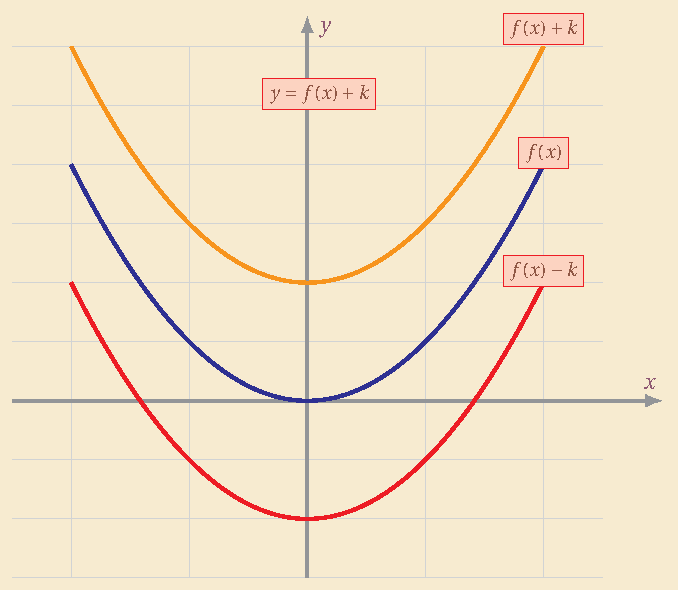
\includegraphics[scale=0.6]
{../mathbook-caos-calculo/images/ej-1-3-3.pdf}%
\caption{Suma de una funci\'{o}n con una constante}%
\label{traslacionejey1}%
\end{figure}


Por su parte, el producto de una funci\'{o}n real $f$ por una funci\'{o}n
constante positiva y diferente de $1$ produce una
\index{Funci\'{o}n!Gr\'{a}fica de una --!Contracci\'{o}n |textit}%
\index{Funci\'{o}n!Gr\'{a}fica de una --!Dilataci\'{o}n|textit}
contracci\'{o}n o una dilataci\'{o}n (\textquotedblleft estiramiento
vertical\textquotedblright) de la gr\'{a}fica de $f$. El producto de $f$ por
$-1$ produce, por su parte una reflexi\'{o}n%
\index{Funci\'{o}n!Gr\'{a}fica de una --!Reflexi\'{o}n|textit}
de la gr\'{a}fica de $f$ con relaci\'{o}n al eje $x$ (ver figura
\ref{contradilata1}).%

\begin{figure}[H]
\centering
\includegraphics[scale=0.8]%
{../mathbook-caos-calculo/images/ej-1-3-4.pdf}%
\caption{Producto de una funci\'{o}n por una constante}%
\label{contradilata1}%
\end{figure}



\paragraph{}

Dado un conjunto no vac\'{\i}o $A$, el conjunto de todas las funciones reales
con dominio $A$ puede dotarse de una \textquotedblleft estructura
algebraica\textquotedblright, definiendo ope\-raciones entre sus elementos. Si
$\rz^{A}$ es el conjunto de tales funciones, entonces para $f,g\in\rz^{A}$, es
claro que $f+g$ y $fg$ son elementos de
\index{a@$(\rz^{A},+,\cdot)$|textbf}%
$\rz^{A}$. La estructura algebraica $(\rz^{A},+,\cdot)$ goza de algunas
propiedades similares a la de la estructura aditivo-multiplicativa de los
reales, algo que no es de extra\~{n}ar, dada la forma como fueron definidas
las operaciones entre funciones.

\begin{theorem}
Sean $f,g,h\in\rz^{A}$. Entonces:

\begin{description}
\item[Leyes asociativas:] $(f+g)+h=f+(g+h)$ y $(fg)h=f(gh)$.

\item[Leyes conmutativas:] $f+g=g+f$ y $fg=gf$.

\item[Existencia de neutros:] Las funciones constantes $O,L\in\rz^{A}$
definidas por
\begin{align}
O(x)  &  =0\\
L(x)  &  =1
\end{align}
satisfacen $f+O=O+f=f$ y $fL=Lf=f$

\item[Existencia de inversos aditivos:] Si $-f=(-1)f$, entonces:
\[
f+(-f)=-f+f=O.
\]

\end{description}
\end{theorem}

\begin{proof}
Las propiedades anteriores son consecuencia de las correspondientes en la
estructura $(\rz,+,\cdot)$. Como ilustraci\'{o}n probemos la asociatividad de
la suma.\newline Para $x\in A$, se tiene que
\begin{align*}
((f+g)+h)(x)  &  =(f+g)(x)+h(x)\\
&  =(f(x)+g(x))+h(x)\\
&  =f(x)+(g(x)+h(x))\\
&  =f(x)+((g+h)(x))\\
&  =(f+(g+h))(x)
\end{align*}
de donde se tiene $(f+g)+h=f+(g+h)$.
\end{proof}

La funci\'{o}n $O$ del teorema anterior es la funci\'{o}n id\'{e}nticamente%
\index{Funci\'{o}n!-- identicamente nula}
nula. Las propiedades listadas en el teorema anterior caracterizan a la
estructura $(\rz^{A},+\cdot)$ como un anillo conmutativo con unidad . Nos
referiremos a el como el \textquotedblleft anillo de funciones reales sobre
$A$\textquotedblright.

\section{Composici\'{o}n de funciones}

Adem\'{a}s de la combinaci\'{o}n de funciones reales (o de funciones con rango
con alguna estructura algebraica) mediante operaciones como la adici\'{o}n y
multiplicaci\'{o}n, podemos tambi\'{e}n \textquotedblleft
conectar\textquotedblright, empalmar o \textquotedblleft
componer\textquotedblright\ dos funciones tales que las im\'{a}genes de una
pertenezcan al dominio de la otra. Para fijar ideas, consideremos funciones
$f$ y $g$ y un elemento $x\in\operatorname*{Dom}(f)$, tal que $f(x)\in
\operatorname*{Dom}(g)$, de modo que $g(f(x))$ est\'{a} definida. Podemos
entonces considerar $g(f(x))$, resultado de las acciones consecutivas de $f$ y
$g$ sobre $x$, como el resultado de una funci\'{o}n a la que denominaremos la
\index{Funci\'{o}n!-- compuesta}%
compuesta de $f$ con $g$. Tal funci\'{o}n ser\'{a} denotada por $g\circ f$. El
esquema siguiente ilustra la situaci\'{o}n.
\[
x\longrightarrow\framebox[2cm]{$f$}\longmapsto f(x)\longmapsto
\framebox[2cm]{$g$}\longmapsto(g\circ f)(x)=g(f(x))
\]
Formalizamos la definici\'{o}n de la operaci\'{o}n composici\'{o}n de funciones.

\begin{definition}
Sean $f:A\longrightarrow B,\ g:C\longrightarrow D$, funciones tales que
$\operatorname*{Ran}(f)\cap\operatorname*{Dom}(g)\neq\emptyset$. La
funci\'{o}n compuesta de $f$ con $g$ es la funci\'{o}n definida por:
\[%
\begin{array}
[c]{cccc}%
\label{compuesta}g\circ f: & \{x\in\operatorname*{Dom}(f)\mid f(x)\in
\operatorname*{Dom}(g)\} & \longrightarrow & D\\
& x & \longmapsto & g(f(x))
\end{array}
\]

\end{definition}

En la definici\'{o}n
\index{Dominio!-- de la funci\'{o}n compuesta}%
anterior, $f$ es denominada la
\index{Funci\'{o}n!-- interna}%
funci\'{o}n interna de la compuesta $g\circ f$. Por supuesto, $g$ es la
funci\'{o}n%
\index{Funci\'{o}n!-- externa}
externa de la compuesta $g\circ f$. N\'{o}tese que si, en particular,
$\operatorname*{Ran}(f)\subseteq\operatorname*{Dom}(g)=C$, entonces
$\operatorname*{Dom}(g\circ f)=\operatorname*{Dom}(f)$. En general, sin
embargo, la composici\'{o}n implica trabajar con restricciones de las
funciones que se componen.

\begin{example}
Debe tenerse cautela al determinar el dominio de una compuesta. Por ejemplo si
$f(x)=x^{2}$ y $g(x)=\sqrt{x}$, para $x$ en el dominio de $g$ se tiene que%
\[
f(g(x))=f(\sqrt{x})=(\sqrt{x})^{2}=x,
\]
lo que podr\'{\i}a llevar a pensar que la compuesta $f\circ g$ es la
funci\'{o}n identidad definida por $I_{\rz}(x)=x$, cuyo dominio es $\rz$. Es
claro, sin embargo, que la compuesta es solo la restricci\'{o}n de la
identidad al conjunto de los reales no negativos, restricci\'{o}n impuesta por
el dominio de la funci\'{o}n interna $g$.
\end{example}

\begin{example}
Por otra parte, se tiene que
\[
(g\circ f)(x)=\sqrt{x^{2}}=|x|,\mbox{ \ para todo real \ }x.
\]

\end{example}

\begin{remark}
N\'{o}tese que al componer dos funciones, realmente se consideran
restricciones adecuadas de las mismas. As\'{\i}, la compuesta de $f$ con $g$
coincide con la de las restricciones
\[
f|_{\{x\in\operatorname*{Dom}(f)\mid f(x)\in\operatorname*{Dom}(g)\}}%
,g|_{\operatorname*{Ran}(f)\cap\operatorname*{Dom}(g)}.
\]
Por lo que, sin p\'{e}rdida de generalidad, podemos suponer en la
definici\'{o}n de compuesta que $f$ y $g$ son funciones
\[
f:X\longrightarrow Y,\ \ g:Y\longrightarrow Z
\]
y que la compuesta de $f$ con $g$ est\'{a} dada por
\[%
\begin{array}
[c]{cccc}%
g\circ f: & X & \longrightarrow & Z\\
& x & \longmapsto & g(f(x))
\end{array}
\]

\end{remark}

\paragraph{}

Para un conjunto cualquiera no vac\'{\i}o $X$, denotamos por $I_{X}$, a la
funci\'{o}n identidad%
\index{Funci\'{o}n!-- identidad}
en $X$, definida por
\begin{equation}
I_{X}(x)=x,\mbox{ \ para todo \ }x\in X \label{identidadX}%
\end{equation}
El siguiente teorema muestra que la composici\'{o}n es una operaci\'{o}n
asociativa y que existen elementos neutros \textquotedblleft
unilaterales\textquotedblright\ para la misma operaci\'{o}n.

\begin{theorem}
\label{compuestaasociativa} Sean $f:X\longrightarrow Y,g:Y\longrightarrow
Z,h:Z\longrightarrow W$ funciones. Entonces:
\begin{equation}
h\circ(g\circ f)=(h\circ g)\circ f \label{asociacompuesta}%
\end{equation}%
\begin{equation}
f\circ I_{X}=I_{Y}\circ f=f \label{neutrocompuesta}%
\end{equation}

\end{theorem}

\begin{proof}
\hfil


\begin{enumerate}
\item Sea $x\in X$, entonces:
\begin{align*}
(h\circ(g\circ f))(x)  &  =h((g\circ f)(x))\\
&  =h(g(f(x))\\
&  =(h\circ g)(f(x))\\
&  =((h\circ g)\circ f)(x)
\end{align*}
Se tiene as\'{\i} que $h\circ(g\circ f)=(h\circ g)\circ f$.

\item Para $x\in X$ tenemos que
\begin{align*}
(f\circ I_{X})(x)  &  =f(I_{X}(x))\\
&  =f(x)\\
&  =I_{Y}(f(x))\\
&  =(I_{Y}\circ f)(x)
\end{align*}
lo que demuestra (\ref{neutrocompuesta}).
\end{enumerate}
\end{proof}

La ecuaci\'{o}n \ref{asociacompuesta} establece la asociatividad de la
composici\'{o}n. Por su parte (\ref{neutrocompuesta}) nos dice que $I_{X}$ es
un neutro \textquotedblleft a derecha\textquotedblright\ para funciones de $X$
a $Y$ y que $I_{Y}$ es un neutro \textquotedblleft a
izquierda\textquotedblright\ para las mismas funciones.

\begin{example}
Consideremos la funci\'{o}n real $f$ definida por
\[
f(x)=x^{2},\mbox{ \ para todo \ }x\in\rz.
\]
Claramente, $f$ no es una funci\'{o}n uno-a-uno, pues para todo real positivo
$y$, la ecuaci\'{o}n $f(x)=x^{2}=y$ tiene dos soluciones distintas $-\sqrt{y}$
y $\sqrt{y}$. Si consideramos la restricci\'{o}n $f|_{\left[  0,+\infty
\right[  }$, \'{e}sta resulta, en cambio, ser inyectiva. La relaci\'{o}n
inversa
\[
g=\{(y,x)\mid(x,y)\in{f\mid}_{\left[  0,+\infty\right[  }\}=\{(y,\sqrt{y})\mid
y\in\left[  0,+\infty\right[  \}
\]
es entonces una funci\'{o}n, pues cada real no negativo $y$ tiene una
\'{u}nica im\'{a}gen. Tal funci\'{o}n es entonces
\[%
\begin{array}
[c]{cccc}%
g: & \left[  0,+\infty\right[  & \longrightarrow & \left[  0,+\infty\right[ \\
& x & \longmapsto & \sqrt{x}%
\end{array}
\]
\textquestiondown Cu\'{a}l es la funci\'{o}n compuesta de la restricci\'{o}n
de $f$ considerada con la funci\'{o}n $g$?\newline Para un real no negativo
$x$ (es decir, en el dominio de la restricci\'{o}n) se tiene:
\begin{align*}
(g\circ f)(x)  &  =g(f(x))\\
&  =g(x^{2})\\
&  =\sqrt{x^{2}}\\
&  =|x|\\
&  =x\\
&  ={I}_{\left[  0,+\infty\right[  }(x)
\end{align*}
De manera similar, se tiene para un $x$ en el dominio de $g$ :
\begin{align*}
(f\circ g)(x)  &  =f(g(x))\\
&  =f(\sqrt{x})\\
&  =\left(  \sqrt{x}\right)  ^{2}\\
&  =x\\
&  =I_{[0,+\infty)}(x);
\end{align*}
Tenemos as\'{\i} que
\[
(g\circ f)(x)=(f\circ g)(x)=I(x),\mbox{ \ para todo \ }x\in\left[
0,+\infty\right[  ,
\]
es decir
\[
f\circ g=g\circ f=I_{\left[  0,+\infty\right[  }%
\]
en el conjunto . Decimos entonces que $g$ es una inversa de $f$ en el conjunto
$\left[  0,+\infty\right[  $. A continuaci\'{o}n formalizamos las definiciones
de funci\'{o}n invertible y de funci\'{o}n inversa.
\end{example}

\begin{definition}
\label{relacioninversa} Sea $R$ una relaci\'{o}n, la
\index{Relaci\'{o}n!-- inversa}%
relaci\'{o}n inversa (o dual) de $R$ es la relaci\'{o}n
\begin{equation}
R^{\ast}=\{(x,y)\mid(y,x)\in R\} \label{ecrelacioninversa}%
\end{equation}
Una funci\'{o}n $f:A\longrightarrow B$ se denomina invertible%
\index{Funci\'{o}n!-- invertible}
si, y solo si la relaci\'{o}n inversa $f^{\ast}$ es tambi\'{e}n una funci\'{o}n.
\end{definition}

Se siguen de la definici\'{o}n

\begin{theorem}
\label{caracterizainversa} Sea $f:A\longrightarrow B$ una funci\'{o}n. Son equivalentes:

\begin{enumerate}
\item $f$ es invertible.

\item $f$ es uno-a-uno.%
\index{Funci\'{o}n!-- inyectiva}%


\item Existe una funci\'{o}n $g:\operatorname*{Ran}(f)\longrightarrow A$, tal
que
\begin{equation}
g\circ f=I_{A},f\circ g=I_{\operatorname*{Ran}(f)}%
\end{equation}

\end{enumerate}
\end{theorem}

\begin{proof}
\hfill

\begin{enumerate}
\item Supongamos que $f$ es invertible y demostremos que es uno-a-uno.
Te\-nemos que $f^{\ast}=\{(x,y)\mid(y,x)\in f\}$ es una funci\'{o}n, por lo
que para todo $x\in\operatorname*{Ran}(f)$, existe una \'{u}nica im\'{a}gen
$y=f^{\ast}(x)$; es decir existe un \'{u}nico $y\in A$ tal que $f(y)=x$. Esto
muestra que $f$ es uno-a-uno.

\item Rec\'{\i}procamente, supongamos que $f$ es uno-a-uno y demostremos ahora
que la relaci\'{o}n inversa $f^{\ast}$ es una funci\'{o}n. Puesto que el
dominio de $f^{\ast}$ es el rango de $f$, consideremos $x\in
\operatorname*{Ran}(f)$. Por la inyectividad de $f$ se sigue que $x$ tiene una
\'{u}nica preim\'{a}gen $y$, o sea $x=f(y)$; as\'{\i}, existe un \'{u}nico
$y\in A$ tal que $(x,y)\in f^{\ast}$. Tenemos as\'{\i} que cada elemento del
dominio de $f^{\ast}$ tiene im\'{a}gen \'{u}nica y, por tanto, $f^{\ast}$ es
una funci\'{o}n. Tomando $g=f^{\ast}$, entonces para $x\in A$ se tiene
\begin{align*}
(x,f(x))\in f  &  \Longrightarrow(f(x),x)\in f^{\ast}\\
&  \Longrightarrow f^{\ast}(f(x))=x\\
&  \Longrightarrow(g\circ f)(x)=I_{A}(x)
\end{align*}
De manera similar, para $x\in\operatorname*{Ran}(f)$, existe $y\in A$ tal que
$x=f(y)$, por lo que $(x,y)\in f^{\ast}$. Se tiene entonces
\begin{align*}
x  &  =f(y)\\
&  =f(f^{\ast}(x))\\
&  =f(g(x))
\end{align*}
de donde se sigue que $f\circ g=I_{\operatorname*{Ran}(f)}$.

\item Para completar la demostraci\'{o}n consideremos ahora que existe una
funci\'{o}n $g$ con las condiciones dadas en el item $3$ del teorema.
Mostremos entonces que la relaci\'{o}n inversa $f^{\ast}$, como conjunto de
pares ordenados, es la misma funci\'{o}n $g$. Consideremos un par ordenado
$(x,y)$. Entonces:
\begin{align*}
(x,y)\in g  &  \Longrightarrow y=g(x)\\
&  \Longrightarrow f(y)=f(g(x))=x\\
&  \Longrightarrow(y,x)\in f\\
&  \Longrightarrow(x,y)\in f^{\ast}%
\end{align*}
Tambi\'{e}n se tiene
\begin{align*}
(x,y)\in f^{\ast}  &  \Longrightarrow(y,x)\in f\\
&  \Longrightarrow x=f(y)\\
&  \Longrightarrow g(x)=g(f(y))=y\\
&  \Longrightarrow(x,y)\in g
\end{align*}
Como $f^{\ast}=g$, se sigue que $f^{\ast}$ es una funci\'{o}n y que $f$ es invertible.
\end{enumerate}
\end{proof}

\paragraph{}

Si $f:A\longrightarrow B$ es una funci\'{o}n invertible, su inversa ser\'{a}
simbolizada por $f^{-1}$. Consideremos un punto $P(x,f(x))$ de la gr\'{a}fica
de $f$. Entonces se tiene que $Q(f(x),x)$ es un punto de la gr\'{a}fica de
$f^{-1}$. La figura \ref{simetriarectaidentidad}, muestra que tales puntos son
v\'{e}rtices opuestos de un cuadrado, con una de sus diagonales sobre la recta
de ecuaci\'{o}n $y=x$.%

\begin{figure}[H]
\centering
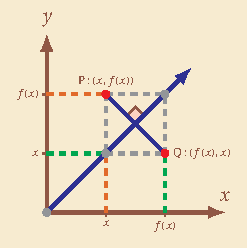
\includegraphics[scale=1.5]{../mathbook-caos-calculo/images/fig-1-5.pdf}%
\caption{Simetr\'{\i}a con relaci\'{o}n a $y=x$}%
\label{simetriarectaidentidad}%
\end{figure}



Es decir, tales puntos son sim\'{e}tricos respecto de dicha diagonal. Se sigue
que las gr\'{a}fica de $f^{-1}$ es la reflexi\'{o}n de la de $f$ con
relaci\'{o}n a la recta de ecuaci\'{o}n $y=x$ (ver figura \ref{finversa1}).

\begin{figure}[H]
\centering
\includegraphics[scale=1]%
{../mathbook-caos-calculo/images/fig-1-6.pdf}%
\caption{Funci\'{o}n inversa}%
\label{finversa1}%
\end{figure}


%TODO
\paragraph{}

El teorema \ref{caracterizainversa} establece que una funci\'{o}n es
invertible si, y solo si es 1-1. Sin embargo, una funci\'{o}n $f$ que no sea
inyectiva puede restringirse en su dominio\footnote{Si, por ejemplo, para
$y\in Ran(f)$ existen m\'{a}s de una \textquotedblleft pre-im\'{a}gen" de $y$,
podemos escoger una sola de estas y restringir el dominio de $f$ escogiendo
una sola preim\'{a}gen de cada elemento del rango, de forma que la
restricci\'{o}n resultante sea inyectiva} de manera tal que la restricci\'{o}n
escogida sea uno-a-uno. Tal restricci\'{o}n ser\'{a} entonces invertible y
diremos que su inversa es una \textquotedblleft inversa de $f$ en el dominio
de la restricci\'{o}n\textquotedblright.

\section{Sucesiones y series de n\'{u}meros reales}

Un caso particular de funciones reales es de inter\'{e}s en esta secci\'{o}n.
Informalmente hablando, una
\index{Sucesi\'{o}n|textbf}%
sucesi\'{o}n en un conjunto cualquiera no vac\'{\i}o $A$ es una funci\'{o}n
con valores sobre ese conjunto y cuya variable recorre un conjunto infinito de
n\'{u}meros enteros no negativos consecutivos. Precisando el concepto, si
$n_{o}$ es un entero no negativo (un n\'{u}mero natural) y $J=\{n\in\nz\mid
n\geq n_{0}\}$, entonces una funci\'{o}n
\[
\alpha:J\longrightarrow A
\]
se denomina una sucesi\'{o}n en o sobre el conjunto $A$. Si $A=\rz$, decimos
que $\alpha$ es una sucesi\'{o}n de n\'{u}meros reales o, m\'{a}s brevemente,
una sucesi\'{o}n real.

\begin{definition}
Sean $n_{0}\in\nz_{0}$. Una funci\'{o}n
\[
\alpha:J=\{n\in\nz\mid n\geq n_{0}\}\longrightarrow\rz
\]
es denominada sucesi\'{o}n real.
\end{definition}

En las condiciones de la definici\'{o}n anterior, la sucesi\'{o}n $\alpha$
ser\'{a} descrita generalmente por sus im\'{a}genes. En ese sentido, la
notaci\'{o}n $\{\alpha(n)\}_{n=n_{0}}^{\infty}$ o $\{\alpha(n)\}_{n\in J}$ se
utilizar\'{a} para referirse a la sucesi\'{o}n $\alpha$. El rango de la
sucesi\'{o}n, es decir el conjunto
\[
\{\alpha(n_{0}),\alpha(n_{0}+1),\alpha(n_{0}+2),\dots\},
\]
puede ser un conjunto finito o infinito. En todo caso, si bien formalmente
hablando la sucesi\'{o}n es la funci\'{o}n $\alpha$, nuestro inter\'{e}s
estar\'{a} centrado en dicho rango, puesto de relieve por la notaci\'{o}n. Se
acostumbra a decir que cada im\'{a}gen $\alpha(n)$ es un t\'{e}rmino de la
sucesi\'{o}n $\alpha$.

\begin{example}
La sucesi\'{o}n real $\alpha:\nz\longrightarrow\rz$, definida por
\[
\alpha(n)=\frac{1}{n}%
\]
ser\'{a} notada como
\[
\left\{  \frac{1}{n}\right\}  _{n\in\nz}.
\]
As\'{\i}, la sucesi\'{o}n considerada toma los valores reales
\[
\left\{  1,\frac{1}{2},\frac{1}{3},\frac{1}{4},\dots\right\}  .
\]
N\'{o}tese que el mismo conjunto de valores es recorrido por las sucesiones
\[
\left\{  \frac{1}{n+1}\right\}  _{n\in\nz_{0}},
\]%
\[
\left\{  \frac{1}{n-1}\right\}  _{n=2}^{\infty},
\]%
\[
\left\{  \frac{1}{n-5}\right\}  _{n=6}^{\infty},
\]
por lo que las sucesiones consideradas podr\'{\i}an considerarse iguales, en
el sentido que producen los mismos valores en el \textquotedblleft mismo
orden\textquotedblright.
\end{example}

\paragraph{}

Precisando la idea del ejemplo anterior, dada una sucesi\'{o}n cualquiera
$\{\alpha(n)\}_{n=n_{0}}^{\infty}$, la funci\'{o}n

\begin{center}
\begin{tabular}
[c]{cccc}%
$f:$ & $\nz$ & $\longrightarrow$ & $J=\{n\in\gz\mid n\geq n_{0}\}$\\
& $1$ & $\longmapsto$ & $n_{0}$\\
& $2$ & $\longmapsto$ & $n_{0}+1$\\
& $3$ & $\longmapsto$ & $n_{0}+2$\\
& $\Vdots$ & $\Vdots$ & $\Vdots$\\
& $n$ & $\longmapsto$ & $n_{0}+(n-1)$\\
&  &  &
\end{tabular}
\end{center}


es biyectiva y para cada natural $n$ se tiene que
\begin{center}
\begin{tabular}[c]{ccc}
$(\alpha\circ f)(1)$  & $ = $     &$\alpha(n_{0})$\\
$(\alpha\circ f)(2)$  & $ = $     &$\alpha(n_{0}+1)$\\
$(\alpha\circ f)(3)$  & $ = $     &$\alpha(n_{0}+2)$\\
$\Vdots            $  & $\Vdots$  &$ \Vdots$
\end{tabular}
\end{center}
por lo que los valores de las sucesiones $\beta=\alpha\circ f$ y $\alpha$ son
los mismos, en el mismo orden. N\'{o}tese que el primer t\'{e}rmino de la
sucesi\'{o}n es $\alpha(n_{0})=\beta(1)$. As\'{\i}, sin p\'{e}rdida de
generalidad, podr\'{\i}amos considerar solo sucesiones cuyo dominio es el
conjunto de los n\'{u}meros naturales; es decir, sucesiones
\[
\{x_{n}\}_{n\in\nz},
\]
donde $x_{n}=\alpha(n)$ y $\alpha:\nz\longrightarrow\rz$ es una funci\'{o}n.

\begin{example}
Para la sucesi\'{o}n $\{\sqrt{n+5}\}_{n=4}^{\infty}$, la funci\'{o}n
\[
f:\nz\ni n\longmapsto n+3\in\{n\in\nz\mid n\geq4\}
\]
da origen a la sucesi\'{o}n
\[
\beta(n)=\sqrt{f(n)}=\sqrt{n+8},\mbox{ \ para todo \
}n\in\nz
\]
cuyo rango es el mismo de la sucesi\'{o}n dada.
\end{example}

\begin{example}
La sucesi\'{o}n $\{(-1)^{n}\}_{n\in\nz}$ tiene el rango finito $\{-1,1\}$
\end{example}

Dada una sucesi\'{o}n real $\{x_{n}\}_{n=n_{0}}^{\infty}$, para $n\geq n_{0}$,
definimos la $n-$\'{e}sima suma parcial
\index{Sucesi\'{o}n!a@$n-$\'{e}sima suma parcial}%
de la sucesi\'{o}n dada por
\begin{equation}
s_{n}=x_{n_{0}}+x_{n_{0}+1}+\dots+x_{n}=\sum_{i=n_{0}}^{n}x_{i}
\label{sumaparcial}%
\end{equation}
la sucesi\'{o}n de sumas parciales
\begin{equation}
\{s_{n}\}_{n=n_{0}}^{\infty}=\left\{  \sum_{i=n_{0}}^{n}x_{i}\right\}
_{n=n_{0}}^{\infty} \label{serie}%
\end{equation}
es denominada una serie real%
\index{Sucesi\'{o}n!Serie asociada a una --}%
. Diremos de ella que es la serie asociada a la sucesi\'{o}n dada.

\begin{example}
Las series asociadas a las sucesiones
\[
\{n+1\}_{n\in\nz},\ \left\{  \frac{1}{n}\right\}  _{n\in\nz}%
\ \mbox{ \ y \ }\{(-1)^{n}\}_{n\in\nz_{0}}%
\]
son, respectivamente
\begin{align*}
\left\{  \sum_{i=1}^{n}(i+1)\right\}  _{n\in\nz}  &
=\{2,2+3,2+3+4,2+3+4+5,\dots\}\\
&  =\{2,5,9,14,\dots\}\\
\left\{  \sum_{i=1}^{n}\frac{1}{i}\right\}  _{n\in\nz}  &  =\left\{
1,1+\frac{1}{2},1+\frac{1}{2}+\frac{1}{3},1+\frac{1}{2}+\frac{1}{3}+\frac
{1}{4},\dots\right\} \\
&  =\left\{  1,\frac{3}{2},\frac{11}{6},\frac{25}{12},\dots\right\} \\
\left\{  \sum_{i=0}^{n}(-1)^{i}\right\}  _{n\in\nz_{0}}  &
=\{1,1+(-1),1+(-1)+1,1+(-1)+1+(-1),\dots\}\\
&  =\{1,0,1,0,\dots\}
\end{align*}

\end{example}

\begin{example}
Para un real fijo $x\neq0$ la sucesi\'{o}n $\{x^{n}\}_{n\in\nz_{0}}$, da
origen a la denominada serie geom\'{e}trica
\begin{equation}
\left\{  \sum_{i=n}^{n}x^{i}\right\}  _{n\in\nz_{0}}=\{1,1+x,1+x+x^{2},\dots\}
\end{equation}
Para $x=0$, la serie geom\'{e}trica est\'{a} determinada por la sucesi\'{o}n
\[
\alpha(n)=%
\begin{cases}
1, & \text{si $n=0$}\\
0^{n}=0, & \text{ si $n>0$}%
\end{cases}
\]
Es decir, el recorrido de la serie geom\'{e}trica es
\[
\{1,1+0,1+0+0,\dots\}.
\]

\end{example}

\paragraph{}

Se acostumbra a escribir
\[
\sum_{n=n_{0}}^{\infty}x_{n}%
\]
para la serie
\[
\left\{  \sum_{i=n_{0}}^{n}x_{i}\right\}  _{n=n_{0}}^{\infty}%
\]


%%%%%%%%%%%%%%%%%%%%%%%%%%%%%%%%%%%%%%%%%%%%%%%%%%%%%%%%%%%%%%%%%%%%%%%%%%%%%%%%%


\section{Ejercicios resueltos}

\begin{example}
Sean $A=\left\{  1,3,-2,5\right\}  $ y $B=\left\{  0,3,2,-1,4\right\}  $ y las
relaciones $R_{k}:A\longrightarrow B,$ $k=1,\ldots,5,$definidas por:
\begin{align*}
R_{1}  &  =\left\{  \left(  1,2\right)  ,\left(  3,3\right)  ,\left(
-2,4\right)  \right\} \\
R_{2}  &  =\left\{  \left(  1,2\right)  ,\left(  3,0\right)  ,\left(
-2,-1\right)  ,\left(  5,4\right)  \right\} \\
R_{3}  &  =\left\{  \left(  3,4\right)  ,\left(  -2,4\right)  ,\left(
1,4\right)  ,\left(  5,4\right)  \right\} \\
R_{4}  &  =\left\{  \left(  -2,0\right)  ,\left(  5,3\right)  ,\left(
3,-1\right)  ,\left(  1,2\right)  ,\left(  3,4\right)  \right\} \\
R_{5}  &  =A\times B
\end{align*}
Determine para cada caso el dominio y el rango, e indique si es funci\'{o}n.
\end{example}

\begin{sol}
El dominio y el rango en cada caso vienen dados por
\[%
\begin{array}
[c]{lll}%
\operatorname*{Dom}\left(  R_{1}\right)  =\left\{  1,3,-2\right\}  &  &
\operatorname*{Ran}\left(  R_{1}\right)  =\left\{  2,3,4\right\} \\
\operatorname*{Dom}\left(  R_{2}\right)  =A &  & \operatorname*{Ran}\left(
R_{2}\right)  =\left\{  4\right\} \\
\operatorname*{Dom}\left(  R_{3}\right)  =A &  & \operatorname*{Ran}\left(
R_{3}\right)  =\left\{  2,0,-1,4\right\} \\
\operatorname*{Dom}\left(  R_{4}\right)  =A &  & \operatorname*{Ran}\left(
R_{4}\right)  =B\\
\operatorname*{Dom}\left(  R_{5}\right)  =A &  & \operatorname*{Ran}\left(
R_{5}\right)  =B
\end{array}
\]
Analizando esta informaci\'{o}n se observa que s\'{o}lo las relaciones $R_{2}$
y $R_{3}$ son funciones, ya que tienen como dominio a $A$ y cada elemento del
dominio tiene imagen \'{u}nica.

$R_{1}$ no es una funci\'{o}n por que $\operatorname*{Dom}\left(
R_{1}\right)  \neq A.$ $R_{4}$ y $R_{5}$ no son funciones porque existen
elementos del dominio que no tienen una \'{u}nica imagen. Por ejemplo $\left(
3,-1\right)  $ y $\left(  3,4\right)  $ en $R_{4},$ y $\left(  1,0\right)  $ y
$\left(  1,3\right)  $ en $R_{5}$.
\end{sol}

\begin{example}
Consideremos las funciones $f$ y $g$ definidas a continuaci\'{o}n:
\[%
\begin{array}
[c]{ccccccccc}%
f: & \rz & \longrightarrow & \rz & \,\,\, & g: & \rz & \longrightarrow & \rz\\
& x & \longmapsto & x^{2}+x+1 & \,\,\, &  & x & \longmapsto & 2x+3
\end{array}
.
\]
Determine para cada una si son uno a uno o sobreyectiva. Adem\'{a}s calcule el
Rango de las funciones.
\end{example}

\begin{sol}
Tenemos que $f(x)=x^{2}+x+1$ para todo real $x$. $f$ no es sobreyectiva, pues
dado un real $y$, la ecuaci\'{o}n cuadr\'{a}tica
\[
x^{2}+x+1=y,\ \mbox{ \ es decir, \ }x^{2}+x+(1-y)=0
\]
solo tiene soluciones reales si, y solo si el discriminante $1-4(1)(1-y)=4y-3$
es no negativo. Ahora
\[
4y-3\geq0\Longleftrightarrow y\geq\frac{3}{4},
\]
lo que muestra que $\operatorname*{Ran}(f)=\left[  \frac{3}{4},\infty\right[
$. As\'{\i}, por ejemplo, no existe un real $x$ tal que $f(x)=x^{2}+x+1=0$.
Por otra parte para $y>\frac{3}{4}$, la ecuaci\'{o}n cuadr\'{a}tica
considerada tiene dos soluciones distintas, por lo que para un tal valor de
$y$ existen dos elementos distintos del dominio cuya im\'{a}gen es la misma,
$y$. Considere, como ilustraci\'{o}n, $y=1$; se tiene entonces
\[
f(x)=x^{2}+x+1=1\Longleftrightarrow x=0\vee x=-1.
\]
Esto muestra que $f$ no es uno-a-uno.

Para $g$ tenemos que dado un real $y$, la ecuaci\'{o}n lineal
\[
g(x)=2x+3=y
\]
tiene siempre soluci\'{o}n \'{u}nica $x=\frac{y-3}{2}$. La existencia de
soluci\'{o}n muestra que la funci\'{o}n es sobre; es decir
$\operatorname*{Ran}(g)=\rz$. El que la soluci\'{o}n sea \'{u}nica indica que
$g$ es uno-a-uno. As\'{\i}, $g$ es una funci\'{o}n biyectiva.
\end{sol}

\begin{example}
Determine el v\'{e}rtice y el rango de $f(x)=x^{2}+3x+2$. Analice la
gr\'{a}fica de la funci\'{o}n.
\end{example}

\begin{sol}
La funci\'{o}n cuadr\'{a}tica dada por $f(x)=x^{2}+3x+2$, tiene una
gr\'{a}fica con v\'{e}rtice en
\[
V\left(  -\frac{3}{2},\frac{8-9}{4}\right)  =V\left(  -\frac{3}{2},-\frac
{1}{4}\right)  ,
\]
por lo que su rango es $\left[  -\frac{1}{4},+\infty\right[  $. El eje de
simetr\'{\i}a es la recta de ecuaci\'{o}n $x=-\frac{3}{2}$. Para trazar un
esbozo a mano de la gr\'{a}fica podemos considerar algunos valores de $x$
menores que $-\frac{3}{2}$; puntos sim\'{e}tricos a cada punto con abscisa $x$
tendr\'{a}n abscisas con valor igual al de $x$ m\'{a}s su distancia al eje de
simetr\'{\i}a. Las ordenadas de puntos sim\'{e}tricos son las mismas. Una
tabla de algunos valores de $x$ e $y$ para la gr\'{a}fica se muestra a
continuaci\'{o}n.
\[%
\begin{tabular}
[c]{|c||c|c|c|c|c|}\hline
$x$ & $-3/2$ & $-5/2,-1/2$ & $-7/2,1/2$ & $-9/2,3/2$ & $-11/2,5/2$\\\hline
$y=f(x)$ & $-\frac{1}{4}$ & $3/4$ & $15/4$ & $35/4$ & $63/4$\\\hline
\end{tabular}
\ \ \ \ \ \ \
\]
Una gr\'{a}fica con computador se muestra en la figura \ref{ejemplopa1}%
\newline%

\begin{figure}[H]
\centering
\includegraphics[scale=0.7]%
{../mathbook-caos-calculo/images/fig-1-7.pdf}%
\caption{Gr\'{a}fica de $f(x)=x^{2}+2x+3$}%
\label{ejemplopa1}%
\end{figure}


\end{sol}
%TODO 
\begin{example}
Sea la funci\'{o}n $y=f(x)=-3\sqrt{4-x^{2}}$

\begin{enumerate}
\item Hallar el dominio.

\item Calcular el rango.

\item Hallar $\dfrac{f\left(  x+h\right)  -f\left(  x\right)  }{h}$
\end{enumerate}
\end{example}

\begin{sol}
\begin{enumerate}
\item Para calcular el dominio de la funci\'{o}n $f,$ se tiene en cuenta que
\begin{align*}
\operatorname*{Dom}f  &  =\left\{  x\in\rz\mid4-x^{2}\geq0\right\} \\
&  =\left\{  x\in\rz\mid4\geq x^{2}\right\} \\
&  =\left\{  x\in\rz\mid\left\vert x\right\vert =\sqrt{x^{2}}\leq\sqrt
{4}\right\} \\
&  =\left\{  x\in\rz\mid-2\leq x\leq2\right\}  =\left[  -2,2\right]
\end{align*}


\item Para obtener el \ rango, observe que para $x\in\left[  -2,2\right]
,y=-3\sqrt{4-x^{2}}\leq0.$ Es decir
\begin{equation}
y\in\left]  -\infty,0\right]  \label{a2}%
\end{equation}
Resolviendo la ecuaci\'{o}n anterior para $x$ se tiene
\begin{equation}
x=3\sqrt{4-\left(  \frac{y}{-3}\right)  ^{2}}\implies4-\frac{y^{2}}{9}%
\geq0\ \implies y\in\left[  -6,6\right]  \label{a3}%
\end{equation}
De $\left(  \ref{a2}\right)  $ y $\left(  \ref{a3}\right)  $ se tiene que el
rango de la funci\'{o}n es el intervalo $\left[  -6,0\right]  $

\item Ya que $f\left(  x\right)  =-3\sqrt{4-x^{2}},$ entonces $f\left(
x+h\right)  =-3\sqrt{4-\left(  x+h\right)  ^{2}}.$ Por lo cual,%
\[
\dfrac{f\left(  x+h\right)  -f\left(  x\right)  }{h}=-3\left(  \dfrac
{\sqrt{4-\left(  x+h\right)  ^{2}}-\sqrt{4-x^{2}}}{h}\right)  .
\]
Racionalizando el numerador se tiene que
\begin{align*}
\dfrac{f\left(  x+h\right)  -f\left(  x\right)  }{h}  &  =-3\left(
\dfrac{4-\left(  x+h\right)  ^{2}-\left(  4-x^{2}\right)  }{h\left(
\sqrt{4-\left(  x+h\right)  ^{2}}+\sqrt{4-x^{2}}\right)  }\right) \\
&  =-3\left(  \dfrac{-h\left(  2x+h\right)  }{h\left(  \sqrt{4-\left(
x+h\right)  ^{2}}+\sqrt{4-x^{2}}\right)  }\right) \\
&  =3\left(  \dfrac{2x+h}{\left(  \sqrt{4-\left(  x+h\right)  ^{2}}%
+\sqrt{4-x^{2}}\right)  }\right)  .
\end{align*}

\end{enumerate}
\end{sol}

\begin{example}
Sea $f(x)=\dfrac{x\sqrt{x^{2}-1}}{x^{2}-x-12}.$ Determine el dominio de la funci\'{o}n
\end{example}

\begin{sol}
Definamos $g\left(  x\right)  :=x\sqrt{x^{2}-1}$ y $h\left(  x\right)
:=x^{2}-x-12.$ Entonces $f\left(  x\right)  $ se puede expresar como el
cociente de estas dos funciones, es decir $f\left(  x\right)  =\dfrac{g\left(
x\right)  }{h\left(  x\right)  }$, por lo tanto%
\begin{equation}
\operatorname*{Dom}\left(  f\right)  =\operatorname*{Dom}\left(  g\right)
\cap\operatorname*{Dom}\left(  h\right)  -\left\{  x\mid h\left(  x\right)
=0\right\}  . \label{fgh}%
\end{equation}
A continuaci\'{o}n calculamos cada uno de los conjuntos dados en (\ref{fgh}).

\begin{enumerate}
\item Como $g\left(  x\right)  :=x\sqrt{x^{2}-1},$entonces
\begin{align*}
\operatorname*{Dom}g  &  =\left\{  x\in\rz\mid x^{2}-1\geq0\right\} \\
&  =\left\{  x\in\rz\mid x^{2}\geq1\right\} \\
&  =\left\{  x\in\rz\mid\left\vert x\right\vert =\sqrt{x^{2}}\geq1\right\} \\
&  =\left\{  x\in\rz\mid x\leq-1\vee1\leq x\right\} \\
&  =\left]  -\infty,-1\right]  \cup\left[  1,+\infty\right[
\end{align*}


\item Como $h\left(  x\right)  :=x^{2}-x-12$ es un polinomio, es claro que
$\operatorname*{Dom}h=\rz.$ Adem\'{a}s
\begin{align*}
\left\{  x\in\rz\mid x^{2}-x-12=0\right\}   &  =\left\{  x\in\rz\mid\left(
x+3\right)  \left(  x-4\right)  =0\right\} \\
&  =\left\{  -3,4\right\}
\end{align*}
En conclusi\'{o}n,
\begin{align*}
\operatorname*{Dom}\left(  f\right)   &  =\left(  -\infty,-1\right]
\cup\left[  1,+\infty\right)  \cap\rz-\left\{  -3,4\right\} \\
&  =\left(  -\infty,-1\right]  \cup\left[  1,+\infty\right)  -\left\{
-3,4\right\} \\
&  =\left]  -\infty,-3\right[  \cup\left]  -3,-1\right]  \cup\left[
1,4\right[  \cup\left]  4,+\infty\right[
\end{align*}

\end{enumerate}
\end{sol}

\begin{example}
Sean las funciones
\begin{align*}
f  &  =\left\{  \left(  1,2\right)  ,\left(  a,3\right)  ,\left(  -1,3\right)
,\left(  2,-2\right)  \right\} \\
g  &  =\left\{  \left(  1,4\right)  ,\left(  a,0\right)  ,\left(
-2,-1\right)  ,\left(  3,-3\right)  ,\left(  2,a\right)  \right\}
\end{align*}
Calcule el dominio y rango de $f$ y $g.$ Obtenga adem\'{a}s
$f+g,fg,f/g,g/f,g\circ f,f\circ g$.
\end{example}

\begin{sol}
En virtud a la definici\'{o}n de $f$ y $g$ se tiene que
\[%
\begin{array}
[c]{lll}%
\operatorname*{Dom}\left(  f\right)  =\left\{  1,a,-1,2\right\}  &  &
\operatorname*{Ran}\left(  f\right)  =\left\{  2,3,-2\right\} \\
\operatorname*{Dom}\left(  g\right)  =\left\{  1,a,-2,3,2\right\}  &  &
\operatorname*{Ran}\left(  g\right)  =\left\{  4,0,-1,-3,a\right\}  .
\end{array}
\]
En $\operatorname*{Dom}\left(  f\right)  \cap\operatorname*{Dom}\left(
g\right)  =\left\{  1,a,2\right\}  $ se definen las funciones%
\begin{align*}
f+g  &  =\left\{  \left(  1,6\right)  ,\left(  a,3\right)  ,\left(
2,a-2\right)  \right\} \\
fg  &  =\left\{  \left(  1,8\right)  ,\left(  a,0\right)  ,\left(
2,-2a\right)  \right\}
\end{align*}
y en los conjuntos
\begin{align*}
\operatorname*{Dom}\left(  f\right)  \cap\operatorname*{Dom}\left(  g\right)
-\left\{  x\in\operatorname*{Dom}\left(  g\right)  \mid g\left(  x\right)
=0\right\}   &  =\left\{  1,2\right\} \\
\operatorname*{Dom}\left(  f\right)  \cap\operatorname*{Dom}\left(  g\right)
-\left\{  x\in\operatorname*{Dom}\left(  f\right)  \mid f\left(  x\right)
=0\right\}   &  =\left\{  1,a,2\right\}
\end{align*}
se definen respectivamente%
\begin{align*}
f/g  &  =\left\{  \left(  1,\frac{1}{2}\right)  ,\left(  2,-\frac{2}%
{a}\right)  \right\} \\
g/f  &  =\left\{  \left(  1,2\right)  ,\left(  a,0\right)  ,\left(
2,-\frac{a}{2}\right)  \right\}  .
\end{align*}
Ya que $\operatorname*{Ran}\left(  g\right)  \cap\operatorname*{Dom}\left(
f\right)  =\left\{  -1\right\}  \neq\emptyset$, y $\operatorname*{Ran}\left(
f\right)  \cap\operatorname*{Dom}\left(  g\right)  =\left\{  2,3,-2\right\}
\neq\emptyset,$ entonces $f\circ g$ y $g\circ f$ est\'{a}n bien definidas, y
dadas por%
\begin{align*}
f\circ g  &  =\left\{  \left(  2,-3\right)  \right\} \\
g\circ f  &  =\left\{  \left(  1,a\right)  ,\left(  a,-3\right)  ,\left(
-1,-3\right)  ,\left(  2,-1\right)  \right\}  .
\end{align*}
De lo anterior es obvio que%
\begin{align*}
\operatorname*{Dom}\left(  f\circ g\right)   &  =\{x\in\operatorname*{Dom}%
(g)\mid g(x)\in\operatorname*{Dom}(f)\}=\left\{  2\right\} \\
\operatorname*{Dom}\left(  g\circ f\right)   &  =\{x\in\operatorname*{Dom}%
(f)\mid f(x)\in\operatorname*{Dom}(g)\}=\left\{  1,a,-1,2\right\}  .
\end{align*}

\end{sol}

\begin{example}
Sea $f\left(  x\right)  =\dfrac{x^{2}+1}{x^{2}-3}$, y $g\left(  x\right)
=-\sqrt{x^{2}-1}.$ De una formula para $h(x)=\left(  f\circ g\right)  \left(
x\right)  ,$ y calcule el dominio de $f\circ g$.
\end{example}

\begin{sol}
Si consideramos la compuesta entre $f$ y $g$ se tiene que
\begin{align*}
\left(  f\circ g\right)  \left(  x\right)   &  =\dfrac{\left(  -\sqrt{x^{2}%
-1}\right)  ^{2}+1}{\left(  -\sqrt{x^{2}-1}\right)  ^{2}-3}\overset{%
%TCIMACRO{\QATOP{x\in\operatorname*{Dom}g}{\downarrow}}%
%BeginExpansion
\genfrac{}{}{0pt}{}{x\in\operatorname*{Dom}g}{\downarrow}%
%EndExpansion
}{=}\frac{x^{2}-1+1}{x^{2}-1-3}\\
&  =\frac{x^{2}}{x^{2}-4}.
\end{align*}
Como
\[%
\begin{array}
[c]{cccc}%
g: & \operatorname*{Dom}(g)=\left]  -\infty,-1\right]  \cup\left[
1,+\infty\right[  & \longrightarrow & \rz^{-}\cup\left\{  0\right\} \\
\vspace{-0.2cm} &  &  & \\
& x & \longmapsto & -\sqrt{x^{2}-1}%
\end{array}
\]
y
\[%
\begin{array}
[c]{cccc}%
f: & \operatorname*{Dom}(f)=\rz-\left\{  \pm\sqrt{3}\right\}  &
\longrightarrow & \left]  -\infty,-\frac{1}{3}\right]  \cup\left]
1,+\infty\right[ \\
\vspace{-0.2cm} &  &  & \\
& x & \longmapsto & \dfrac{x^{2}+1}{x^{2}-3},
\end{array}
\]
es claro que la compuesta $f\circ g$ existe, y%
\[
\operatorname*{Dom}\left(  f\circ g\right)  =\{x\in\operatorname*{Dom}(g)\mid
g(x)\in\operatorname*{Dom}(f)\}.
\]
Si $x\in\operatorname*{Dom}\left(  f\circ g\right)  ,$ entonces

\begin{enumerate}
\item $x\in\left]  -\infty,-1\right]  \cup\left[  1,+\infty\right[  ,$ y

\item $g(x)\in\rz-\left\{  \pm\sqrt{3}\right\}  $
\end{enumerate}

De la segunda condici\'{o}n se tiene que $-\sqrt{x^{2}-1}\neq\pm\sqrt{3}.$ Es
claro que $-\sqrt{x^{2}-1}\neq+\sqrt{3},$ por lo tanto nos falta determinar el
conjunto%
\[
\left\{  x\in\operatorname*{Dom}(g)\mid-\sqrt{x^{2}-1}\neq-\sqrt{3}\right\}
=\left]  -\infty,-1\right]  \cup\left[  1,+\infty\right[  -\left\{
x\mid-\sqrt{x^{2}-1}=-\sqrt{3}\right\}
\]


pero $\left\{  x\mid-\sqrt{x^{2}-1}=-\sqrt{3}\right\}  =\left\{  \pm2\right\}
.$ Por lo tanto%

\begin{align*}
\operatorname*{Dom}\left(  f\circ g\right)   &  =\{x\in\operatorname*{Dom}%
(g)\mid g(x)\in\operatorname*{Dom}(f)\}\\
&  =\left(  -\infty,-1\right]  \cup\left[  1,+\infty\right)  -\left\{
\pm2\right\} \\
&  =\left]  -\infty,-2\right[  \cup\left]  -2,-1\right]  \cup\left[
1,2\right[  \cup\left]  2,+\infty\right[
\end{align*}

\end{sol}

\begin{example}
Consideremos las funciones reales definidas por
\[
f(x)=\sqrt{2x+9},\ \ g(x)=\sqrt{x^{2}-x-6}.
\]
Obtenga $\operatorname*{Dom}\left(  f\right)  ,\operatorname*{Dom}\left(
g\right)  ,f+g,fg,\frac{f}{g},\operatorname*{Dom}\left(  f+g\right)
,\operatorname*{Dom}\left(  fg\right)  ,\operatorname*{Dom}\left(  \frac{f}%
{g}\right)  .$
\end{example}

\begin{sol}
Se tiene que:
\begin{align*}
\operatorname*{Dom}(f)  &  =\{x\in\rz\mid2x+9\geq0\}\\
&  =\{x\in\rz\mid x\geq-9/2\}\\
&  =\left[  -\frac{9}{2},+\infty\right[ \\
\operatorname*{Dom}(g)  &  =\{x\in\rz\mid x^{2}-x-6=(x-3)(x+2)\geq0\}\\
&  =\left]  -\infty,-2\right]  \cup\left[  3,+\infty\right[
\end{align*}
Se tiene as\'{\i} que
\[
\operatorname*{Dom}(f)\cap\operatorname*{Dom}(g)=\left[  -\frac{9}%
{2},-2\right]  \cup\lbrack3,+\infty)
\]
conjunto sobre el cual est\'{a}n definidas las funciones
\begin{align*}
(f+g)(x)  &  =\sqrt{2x+9}+\sqrt{x^{2}-x-6}\\
(f-g)(x)  &  =\sqrt{2x+9}-\sqrt{x^{2}-x-6}\\
(fg)(x)  &  =\sqrt{2x^{3}+7x^{2}-21x-54}\\
\left(  \frac{f}{g}\right)  \left(  x\right)   &  =\frac{\sqrt{2x+9}}%
{\sqrt{x^{2}-x-6}}%
\end{align*}
\textquestiondown Por qu\'{e} $\left(  fg\right)  \left(  x\right)
=\sqrt{2x^{3}+7x^{2}-21x-54}$ ?.

Por su parte el cociente $f/g$ est\'{a} definido sobre
\[
\left[  -\frac{9}{2},-2\right[  \cup\left]  3,+\infty\right[
\]
y $g/f$ lo est\'{a} sobre
\[
\left]  -\frac{9}{2},-2\right]  \cup\left[  3,+\infty\right[  .
\]



\end{sol}

\begin{example}
Consideremos las funciones finitas
\begin{align*}
f  &  =\{(a,1),(b,0),(c,2)\}\\
g  &  =\{(1,5),(0,3),(3,6)\}.
\end{align*}
Determine si $g\circ f$ o $f\circ g$ estan bien definidas. En caso afirmativo
determine la compuesta y el dominio respectivo. En caso negativo justifique la respuesta.
\end{example}

\begin{sol}
Ya que $\operatorname*{Ran}(f)\cap\operatorname*{Dom}(g)=\{1,0\}$, entonces
$g\circ f$ est\'{a} definida sobre el conjunto
\[
\{x\in\operatorname*{Dom}(f)\mid f(x)\in\operatorname*{Dom}(g)\}=\{a,b\}.
\]
Adem\'{a}s, se tiene que
\[
g\circ f=\{(a,5),(b,3)\}.
\]
Puesto que $\operatorname*{Ran}(g)\cap\operatorname*{Dom}(f)=\emptyset$ la
compuesta $f\circ g$ no est\'{a} definida.
\end{sol}

\begin{example}
Para las funciones de variable real definidas por:
\[
f(x)=x^{2}+x,\ g(x)=\sqrt{x},
\]
determine $\operatorname*{Dom}\left(  f\right)  ,\operatorname*{Dom}\left(
g\right)  ,\operatorname*{Dom}\left(  g\circ f\right)  ,\operatorname*{Dom}%
\left(  f\circ g\right)  .$ \textquestiondown Las compuestas $f\circ g$ y
$g\circ f$ son iguales?
\end{example}

\begin{sol}
$\operatorname*{Dom}(f)=\rz$, $\operatorname*{Dom}(g)=\left[  0,+\infty
\right[  $. Por lo que
\begin{align*}
x\in\operatorname*{Dom}(g\circ f)  &  \Longleftrightarrow x\in\rz\ \wedge
\ f(x)=x^{2}+x\geq0\\
&  \Longleftrightarrow x(x+1)\geq0\\
&  \Longleftrightarrow x\in\left]  -\infty,-1\right]  \cup\left[
0,+\infty\right[
\end{align*}
Tenemos as\'{\i} que $(g\circ f)(x)=g(x^{2}+x)=\sqrt{x^{2}+x}$, para todo $x$
en el conjunto $\left]  -\infty,-1\right]  \cup\left[  0,+\infty\right[  $.

Por otra parte:
\begin{align*}
x\in\operatorname*{Dom}(f\circ g)  &  \Longleftrightarrow x\in
\operatorname*{Dom}(g)\ \wedge\ g(x)=\sqrt{x}\in\operatorname*{Dom}(f)=\rz\\
&  \Longleftrightarrow x\geq0
\end{align*}
Se tiene as\'{\i} que
\[
(f\circ g)(x)=f(g(x))=(\sqrt{x})^{2}+\sqrt{x}=x+\sqrt{x},\ \mbox{para
todo \ }x\geq0.
\]
N\'{o}tese que $\operatorname*{Ran}(g)\subseteq\operatorname*{Dom}(f)$, por lo
que $\operatorname*{Dom}(f\circ g)=\operatorname*{Dom}(g)$. Debe notarse
tambi\'{e}n que $f\circ g\neq g\circ f$ pues, por ejemplo:
\[
(f\circ g)(1)=2\neq\sqrt{2}=(g\circ f)(1),
\]
lo que muestra que, en general, la composici\'{o}n no es conmutativa.
\end{sol}

\begin{example}
Consideremos la funci\'{o}n
\[
f=\{(1,2),(2,3),(3,3),(4,1)\}
\]
con dominio $A=\{1,2,3,4\}.$ \textquestiondown $f$ es invertible?. En caso
afirmativo obtenga la funci\'{o}n inversa. En caso negativo determine
restricciones de $f$ para las cuales exista inversa.
\end{example}

\begin{sol}
Claramente $f$ no es uno-a-uno y, por tanto, no es invertible, ya que como
$3=f(2)=f(3)$, la relaci\'{o}n inversa
\[
f^{\ast}=\{(2,1),(3,2),(3,3),(1,4)\}
\]
no es una funci\'{o}n pues $3$ tiene dos im\'{a}genes distintas ($2$ y $3$)
bajo $f^{\ast}$. Si restringimos $f$ al conjunto $\{1,2,4\}$ (o a
$\{1,3,4\}$), la restricci\'{o}n resultante ser\'{a} uno-a-uno y, por lo
tanto, invertible. As\'{\i}, una inversa de $f$ es
\[
g=\{(2,1),(3,2),(1,4)\}
\]
en el conjunto $A_{1}=\{1,2,4\}$. Tambi\'{e}n, la funci\'{o}n
$h=\{(2,1),(3,3),(1,4)\}$ es una inversa de $f$, ahora en $A_{2}=\{1,3,4\}$.
Siendo formales, se tiene que:
\begin{align*}
{f^{-1}\mid}_{A_{1}}  &  =g\\
f^{-1}|_{A_{2}}  &  =h
\end{align*}

\end{sol}

\begin{example}
Determine si la funci\'{o}n lineal $f$, definida por
\[
f(x)=2x+3
\]
es invertible. En tal caso calcule $f^{-1}.$
\end{example}

\begin{sol}
Claramente la funci\'{o}n lineal $f$ es uno-a-uno; por lo tanto es invertible.
Para determinar su inversa, tenemos en cuenta que
\[
f=\{(x,y)\mid y=f(x)=2x+3,x\in\rz\}.
\]
Por lo que
\begin{align*}
f^{-1}  &  =f^{\ast}\\
&  =\{(x,y)\mid(y,x)\in f\}\\
&  =\{(x,y)\mid x=2y+3\}\\
&  =\left\{  (x,y)\ \left\vert \ y=\frac{x-3}{2}\right.  \right\}
\end{align*}
Se tiene as\'{\i} que para $x\in\rz$,
\[
f^{-1}(x)=\frac{x-3}{2}.
\]
En efecto, para $x\in\rz$, se tiene
\begin{align*}
f(f^{-1}(x))  &  =f\left(  \frac{x-3}{2}\right) \\
&  =2\left(  \frac{x-3}{2}\right)  +3\\
&  =x\\
&  =I_{\rz}(x)\\
f^{-1}(f(x))  &  =f^{-1}\left(  2x+3\right) \\
&  =\frac{(2x+3)-3}{2}\\
&  =x\\
&  =I_{\rz}(x)
\end{align*}

\end{sol}

\newpage

\section{Ejercicios propuestos}

\begin{enumerate}
\item Determine en cada caso si la gr\'{a}fica representa una
funci\'{o}n.\newline
\begin{figure}[H]
\centering
\subfigure[]{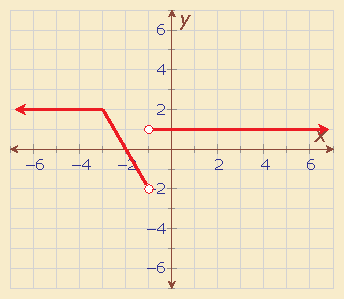
\includegraphics[scale=0.8]{../mathbook-caos-calculo/images/ejp-1-8-1g.pdf}}\hfill%
\subfigure[]{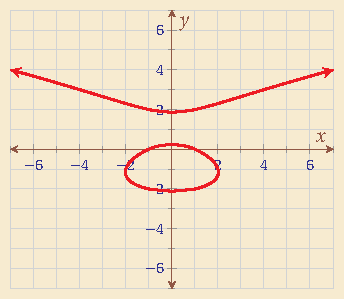
\includegraphics[scale=0.8]{../mathbook-caos-calculo/images/ejp-1-8-1h.pdf}}\hfill%
\subfigure[]{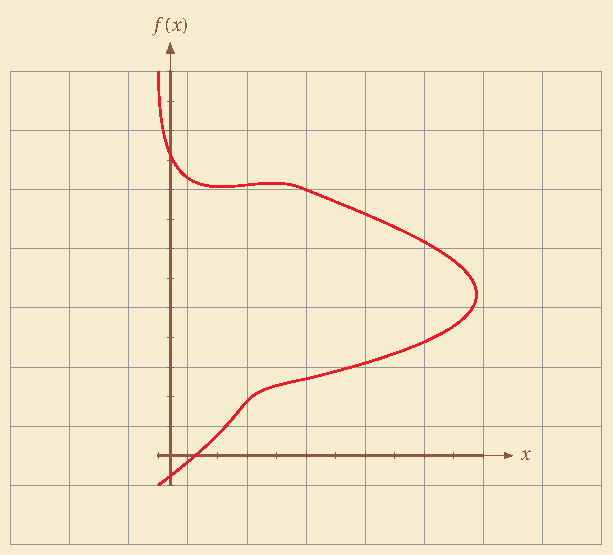
\includegraphics[scale=0.4]{../mathbook-caos-calculo/images/ejp-1-8-1c.pdf}}\\%
\subfigure[]{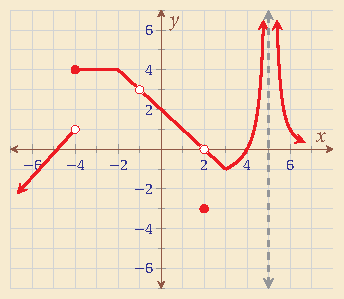
\includegraphics[scale=0.8]{../mathbook-caos-calculo/images/ejp-1-8-1e.pdf}}\hfill%
\subfigure[]{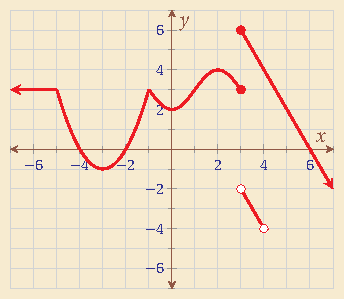
\includegraphics[scale=0.8]{../mathbook-caos-calculo/images/ejp-1-8-1f.pdf}}\hfill%
\subfigure[]{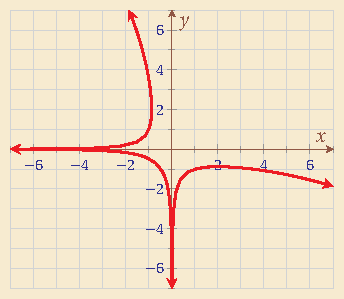
\includegraphics[scale=0.8]{../mathbook-caos-calculo/images/ejp-1-8-1j.pdf}}%
\end{figure}	
	

\item Un punto $P\left(  x,y\right)  $ se mueve, en sentido horario, sobre la
par\'{a}bola
\[
\left(  x-2\right)  ^{2}+16\left(  y+5\right)  =0.
\]
Exprese mediante una funci\'{o}n de variable real la distancia del punto
$P\left(  x,y\right)  $ al punto $A\left(  2,2\right)  .$

\item \label{cap1prob3}Una v\'{\i}a de ferrocarril cruza una carretera
formandose un \'{a}ngulo de $60^{0}$, como lo muestra la figura
\begin{center}
\includegraphics[scale=0.8]%
{../mathbook-caos-calculo/images/ejp-1-3.pdf}%
\end{center}

Una locomotora a $800$ metros de la intersecci\'{o}n se aleja de ella a
raz\'{o}n de $100\dfrac{km}{h}.$ Un automovil a $800$ metros de la
intersecci\'{o}n se acerca a ella a raz\'{o}n de $80\dfrac{km}{h}.$
\textquestiondown Cu\'{a}l es la distancia de separaci\'{o}n entre el
automovil y la locomotora en ese instante ?. Exprese mediante una funci\'{o}n
de variable real, dependiente del tiempo $t$, la distancia de separaci\'{o}n
entre la locomotora y el automovil$.$

\item Cierta cantidad de aceite fluye hacia el interior de un deposito en
forma de cono invertido a raz\'{o}n de $0.1\pi\,\frac{m^{3}}{\min}.$ El
deposito tiene un radio de $2.5m$ en su parte superior y una profundidad de
$10m$. Si el deposito inicialmente contiene $1.2m^{3}$ de aceite. Exprese
mediante una funci\'{o}n de variable real, dependiente de la altura $h$, la
cantidad de aceite del recipiente.%
\begin{center}
\includegraphics[scale=0.6]%
{../mathbook-caos-calculo/images/ejr-1-8-4.pdf}%
\end{center}




\item Sea $\triangle ABC$ is\'{o}sceles con $AB=AC,$ y $m\measuredangle
BAC=\alpha.$ Exprese mediante una funci\'{o}n de variable real, dependiente
del valor del \'{a}ngulo $\alpha,$ el \'{a}rea del $\triangle ABC$.

\item Una isla est\'{a} ubicada en el punto $A$, $4\,km$ mar adentro del punto
m\'{a}s cercano $B$ de una playa recta. Una atleta, en la isla desea ir al
punto $C$, a $6$ $km$ de $B$ playa abajo. La mujer debe dirigirse hacia un
punto $P$, entre $B$ y $C$, en un bote de remos a $3.5\dfrac{km}{h}$ y
desp\'{u}es caminar en forma recta de $P$ a $C$ a $6\dfrac{km}{h}.$ Exprese
mediante una funci\'{o}n de variable real, dependiente de $x=BP,$ el tiempo
necesario para viajar desde $A$ hacia $C,$ pasando por el punto $P$.
\begin{center}
\includegraphics[scale=0.3]%
{../mathbook-caos-calculo/images/ejp-1-6.pdf}%
\end{center}


\item Exprese mediante una funci\'{o}n de variable real, dependiente de $x,$
el \'{a}rea del rect\'{a}ngulo que tiene dos v\'{e}rtices en el eje $x$ y los
otros dos en la par\'{a}bola $y=16-x^{2},$ por arriba del eje $x.$

\item Hay que construir una pileta de las dimensiones que se muestran.
S\'{o}lo se puede variar el \'{a}ngulo $\theta$ . Exprese mediante una
funci\'{o}n de variable real, dependiente del \'{a}ngulo $\theta,$ el volumen
de la pileta.%
\begin{center}
\includegraphics[scale=0.3]%
{../mathbook-caos-calculo/images/ejr-1-8-8.pdf}%
\end{center}


\item Un granjero desea cercar tres terrenos rectangulares adyacentes
identicos, cada uno de ellos de 1800 pies cuadrados de \'{a}rea, incluyendo
cerca en medio de ellos. Exprese mediante una funci\'{o}n de variable real,
dependiente de la profundidad de los terrenos, el perimetro total para
realizar est\'{a} tarea.

\item Dada una esfera de radio $R$. Exprese mediante una funci\'{o}n de
variable real, dependiente de $R$, el volumen del cono circular recto de radio
$r$ y altura $h$ que puede inscribirse en la esfera.

\item Una particula se mueve a lo largo de una l\'{\i}nea recta, siendo su
posici\'{o}n $x\left(  t\right)  $ metros en todo tiempo $t>0$ segundos
\[
x\left(  t\right)  =\dfrac{5t+20}{t+1}+2t
\]


\begin{enumerate}
\item Completa la siguiente tabla:%
\[%
\begin{tabular}
[c]{|l|l|l|l|l|l|l|l|}\hline
$t\left[  s\right]  $ & $1$ & $2$ & $3$ & $4$ & $5$ & $6$ & $7$\\\hline
$x\left[  m\right]  $ &  &  &  &  &  &  & \\\hline
\end{tabular}
\ \
\]


\item Usa los resultados de la tabla para hacer un bosquejo de la gr\'{a}fica
de $x\left(  t\right)  .$ Con la ayuda de un software, gr\'{a}fique $x$ $vs$
$t.$ Compare y analice las gr\'{a}ficas.

\item \textquestiondown En qu\'{e} momento la part\'{\i}cula alcanza una
posici\'{o}n de $3$ metros?
\end{enumerate}

\item Una hoja de papel de dimensiones 12 cms por 8 cms , se corta por las
esquinas en cuadrados de $x$ cms de lado.

\begin{enumerate}
\item Muestre que el volumen que se puede construir a partir de la hoja viene
dado por $V(x)=4x(6-x)(4-x),0<x<4.$

\item Complete la siguiente tabla:%
\[%
\begin{tabular}
[c]{|l|l|l|l|l|l|}\hline
$x$ $\left[  cm\right]  $ & $0$ & $1$ & $2$ & $3$ & $4$\\\hline
$V$ $\left[  cm^{3}\right]  $ &  &  &  &  & \\\hline
\end{tabular}
\ .
\]


\item Estime el m\'{a}ximo volumen que puede tener la caja ( Explique sus procedimientos)
\end{enumerate}

\item Una funci\'{o}n est\'{a} definida por $f(x)=3x+1,$ $x\in R$. Determine
el conjunto soluci\'{o}n de la ecuaci\'{o}n $f(2x)-f(x+1)=4.$

\item Considere los conjuntos
\[
A=\{x\in\nz\mid x<5\},B=\{x\in\nz\mid3\leq x\leq5\}.
\]
Para cada una de las relaciones de $A$ a $B$ dadas a continuaci\'{o}n
determine su dominio y su rango. Haga una gr\'{a}fica de la relaci\'{o}n e
indique si la relaci\'{o}n dada es una funci\'{o}n. En caso de serlo indique
si es sobre, uno-a-uno o biyectiva. Justifique todas sus respuestas.

\begin{enumerate}
\item $R=\{(2,3),(3,5),(1,3),(4,4)\}$.

\item $S=\{(1,3),(2,3),(3,4),(4,5)\}$.

\item $T=\{(1,3),(1,4),(1,5)\}$.

\item $U=\{(1,3),(2,3),(3,3),(4,3)\}$.

\item $V=\{(1,4),(2,3)\}$.
\end{enumerate}

\item Considere, en cada caso, la funci\'{o}n de variable real $f$ definida
por la f\'{o}rmula dada. Determine dominio y rango de la funci\'{o}n e indique
si es sobre, uno-a-uno o biyectiva. Haga una gr\'{a}fica de la funci\'{o}n.
Indique tambi\'{e}n, si los hay, los valores m\'{a}ximo y m\'{\i}nimo de la funci\'{o}n.

\begin{enumerate}
\item $f(x)=x^{2}+3x+2$.

\item $f(x)=3x+7$.

\item $f(x)=3x^{2}+x-4$.

\item $f(x)=-x^{2}+x+1$.

\item $f(x)=\pi$.

\item $f(x)=2x^{2}-3x+5$.

\item $f(x)=|x-2|$.

\item $f(x)=|x^{2}+3x+2|$.
\end{enumerate}

\item Para cada una de las funciones del ejercicio anterior determine las
intersecciones de su gr\'{a}fica con los ejes coordenados. En cada caso
determine el dominio de la funci\'{o}n de variable real definida por la
f\'{o}rmula dada.

\begin{enumerate}
\item $f(x)=\sqrt{x^{2}+5x+6}$.

\item $f(x)=\dfrac{2-x}{x^{2}+5x+6}$.

\item $f(x)=\dfrac{\sqrt{2-x}}{x+3}$.

\item $f(x)=\dfrac{x+1}{3x^{2}+x+1}$.

\item $f(x)=\sqrt{|x|}$.

\item $f(x)=\sqrt{\dfrac{x-1}{2x+3}}$.

\item $f\left(  x\right)  =\sqrt{x^{2}+2x-15}$
\end{enumerate}

\item Considere la funci\'{o}n definida por $g(x)=x^{3}+x^{2}+1$.
\textquestiondown Est\'{a} $3$ en el rango de $g$? \textquestiondown Es $g$
una funci\'{o}n uno-a-uno?

\item Sea $f$ definida por $f(x)=\sqrt{2x+1}$. Encuentre los valores de $h$
para los cuales $2+h$ est\'{a} en:

\begin{enumerate}
\item El dominio de $f$.

\item El rango de $f$.
\end{enumerate}

\item En cada caso indique si la relaci\'{o}n real dada es una funci\'{o}n. En
caso afirmativo indique el dominio de la misma. En caso negativo, encuentre
una funci\'{o}n definida impl\'{\i}citamente por la ecuaci\'{o}n que define la relaci\'{o}n.

\begin{enumerate}
\item $R=\{(x,y)\mid x^{2}-y^{2}=1\}$.

\item $S=\{(x,y)\mid x^{2}+xy-3x=0\}$.

\item $T=\{(x,y)\mid x=1,x^{2}+x-y=0\}$.

\item $U=\{(t,u)\mid t^{2}+u^{2}-2u=0\}$.

\item $V=\{(t,s)\mid s^{3}+2s^{2}+s-t=0\}$.
\end{enumerate}

\item Considere la relaci\'{o}n $R=\{(x,y)\mid Ax^{2}+Cy^{2}+Dx+Ey+F=0\}$,
donde $A,C,D,E$ y $F$ son reales dados. Demuestre que:

\begin{enumerate}
\item Si $A=C\neq0$, la gr\'{a}fica de $R$ es una circunferencia, un punto o
el conjunto vac\'{\i}o.

\item Si $A=0$ o $C=0$, la gr\'{a}fica de $R$ es una par\'{a}bola, dos rectas
paralelas, una sola recta o el conjunto vac\'{\i}o.
\end{enumerate}

\item \label{ejercicio1} En cada caso determine el dominio de $f+g,fg$ y
$f/g$, para las funciones reales $f$ y $g$ definidas como se indica. Encuentre
adem\'{a}s
\[
(f+g)(x),(fg)(x),(f/g)(x)
\]
para $x$ en el dominio de la correspondiente funci\'{o}n.

\begin{enumerate}
\item $f(x)=\dfrac{x}{x-2},\ g(x)=\sqrt{x^{2}-x}$.

\item $f(x)=\dfrac{x-2}{x^{2}-3x+2},\ g(x)=\dfrac{2}{x+1}$.

\item $f(x)=\sqrt{x^{2}+3x+2},\ g(x)=\dfrac{x}{x+2}$.

\item $f(x)=\sqrt{x+1},\ g(x)=\sqrt{x^{2}+x+1}$.

\item $f(x)=\sqrt{\dfrac{x+1}{x-2}},\ g(x)=\sqrt{6+x-x^{2}}$.
\end{enumerate}

\item Como en el ejercicio anterior para las funciones
\[
f=\{(a,0),(b,1),(c,-3),(d,-5)\},\ g=\{(a,3),(b,-5),(c,6),(e,9)\}
\]


\item Sea $f$ la funci\'{o}n de variable real definida por $f(x)=5x+3$.
Determine todos los valores de $x$ para los cuales:

\begin{enumerate}
\item $f(2x)=2f(x)$.

\item $f(x+c)=f(x)+f(c)$, si $c$ es un real fijo dado.\newline Haga lo mismo
si $f(x)=5x$.
\end{enumerate}

\item Sea $f:\rz\longrightarrow\rz$ una funci\'{o}n. $f$ es una
\index{Aplicaci\'{o}n lineal|textbf}%
aplicaci\'{o}n lineal si, y solo si para todo $x_{1},x_{2}\in\rz$ se cumple
que $f(x_{1}+x_{2})=f(x_{1})+f(x_{2})$ y $f(x_{1}x_{2})=x_{1}f(x_{2})$.
Demuestre que el conjunto de todas las aplicaciones lineales de $\rz$ en
$\rz$, al cual notaremos $Lin(\rz,\rz)$, es cerrado para las operaciones de
adici\'{o}n de funciones y multiplicaci\'{o}n por funciones constantes. Es
decir, demuestre que si $f,g\in Lin(\rz,\rz)$ y $k\in\rz$ entonces:
\begin{align*}
(f+g)  &  \in Lin(\rz,\rz)\\
kf  &  \in Lin(\rz,\rz).
\end{align*}


\item Demuestre que una funci\'{o}n $f:\rz\longrightarrow\rz$ es una
aplicaci\'{o}n lineal si, y solo si existe una constante $k\in\rz$ tal que
$f(x)=kx$, para todo $x\in\rz$. As\'{\i}, toda aplicaci\'{o}n lineal es una
funci\'{o}n lineal. \textquestiondown Es verdadero el rec\'{\i}proco?.

\item En cada caso determine, si est\'{a}n definidas, las compuestas $f\circ
g$ y $g\circ f$, indicando sus dominios de definici\'{o}n.

\begin{enumerate}
\item $f=\{(a,1),(2,-3),(c,d),(0,5)\},\ g=\{(1,3),(5,6),(a,4)\}$.

\item $f=\{(3,2),(4,5),(6,7)\},\ g=\{(2,4),(5,6),(8,3)\}$.

\item $f$ y $g$ son funciones de variable real definidas por:

\begin{enumerate}
\item $f(x)=2,\ g(x)=5x$.

\item $f(x)=3,\ g(x)=2$.

\item $f(x)=x+1,\ g(x)=x-1$.

\item $f(x)=x^{2}+2x-3,\ g(x)=\sqrt{x}$.

\item $f(x)=\sqrt{x-2},\ g(x)=x^{3}$.

\item $f(x)=\dfrac{x}{x+3},g(x)=\sqrt{x+1}$.
\end{enumerate}
\end{enumerate}

\item En cada caso indique si la funci\'{o}n dada es invertible. En caso
afirmativo, encuentre su inversa. Si no es invertible, encuentre al menos dos
restricciones de la funci\'{o}n dada que sean invertibles y halle las inversas
de tales restricciones. Utilice software adecuado para graficar la funci\'{o}n
(o una restricci\'{o}n de la misma) y su inversa.

\begin{enumerate}
\item $f=\{(1,3),(\pi,5),(\sqrt{2},3),(5,7)\}$.

\item $g=\{(2,1),(3,5),(4,0),(6,1),(8,5)\}$.

\item La funci\'{o}n de variable real $f$ definida por:

\begin{enumerate}
\item $f(x)=5x-7$.

\item $f(x)=6$.

\item $f(x)=x$.

\item $f(x)=ax+b$, donde $a,b\in\rz$.

\item $f(x)=x^{2}-x-30$.

\item $f(x)=ax^{2}+bx+c$, donde $a,b$ y $c$ son reales cualesquiera con
$a\neq0$.

\item $f(x)=\sqrt{x}$.

\item $f(x)=x^{3}$.
\end{enumerate}
\end{enumerate}

\item Una funci\'{o}n $f:\rz\longrightarrow\rz$ se denomina localmente
invertible si existe un intervalo abierto $\left]  a,b\right[  $ tal que la
restricci\'{o}n $f|_{\left]  a,b\right[  }$ es invertible. En tal caso
$f|_{\left]  a,b\right[  }^{-1}$ es una inversa local de $f$. Encuentre al
menos dos inversas locales para la funci\'{o}n $f$ definida por:

\begin{enumerate}
\item $f(x)=x^{2}+3x+5$.

\item $f(x)=x^{3}$.
\end{enumerate}

\item Sea $f$ una funci\'{o}n real invertible \textquestiondown Se puede
afirmar que $f^{-1}=\dfrac{1}{f}$? Justifique su respuesta.

\item Sea $a$ un real positivo. Una funci\'{o}n $f:[-a,a]\longrightarrow\rz$
se denomina%
\index{Funci\'{o}n!-- par}
par si, y solo si
\[
f(-x)=f(x)\ \mbox{para todo \ }x\in\lbrack-a,a].
\]
$f$ es una funci\'{o}n impar%
\index{Funci\'{o}n!-- impar}
si, y solo si
\[
f(-x)=-f(x)\ \mbox{para todo \ }x\in\lbrack-a,a].
\]


\begin{enumerate}
\item Demuestre que si $f(x)=x^{2}+1$, entonces $f$ es par y que la
funci\'{o}n $g$ definida por $g(x)=x^{3}+x$ es impar.

\item \textquestiondown Es toda funci\'{o}n constante una funci\'{o}n par?

\item Demuestre que una funci\'{o}n lineal es par si, y solo si es constante e
impar si, y solo si es un m\'{u}ltiplo de la funci\'{o}n id\'{e}ntidad. En
particular, la funci\'{o}n identidad es impar.

\item Demuestre que la funci\'{o}n cuadr\'{a}tica $f(x)=ax^{2}+bx+c$ es una
funci\'{o}n par si, y solo si $b=0$. \textquestiondown Existen funciones
cuadr\'{a}ticas impares?.

\item Discuta la veracidad de la siguiente afirmaci\'{o}n:

Si $f$ es una funci\'{o}n par, su gr\'{a}fica es sim\'{e}trica respecto del
eje $Y$.
\end{enumerate}

\item En cada caso indique si la proposici\'{o}n dada es Verdadera o falsa.
Justifique sus respuestas.

\begin{enumerate}
\item Toda funci\'{o}n lineal es invertible.

\item Una funci\'{o}n lineal es invertible si, y solo si no es constante.

\item Toda funci\'{o}n lineal no constante es localmente invertible.

\item Toda funci\'{o}n cuadr\'{a}tica es invertible.

\item Ninguna funci\'{o}n cuadr\'{a}tica es invertible.

\item Toda funci\'{o}n cuadr\'{a}tica es localmente invertible.

\item Una funci\'{o}n real de variable real es invertible si, y solo si toda
recta paralela al eje $X$ que intersecte su gr\'{a}fica lo hace en un solo punto.

\item Una funci\'{o}n $f:\rz\longrightarrow\rz$ es par si, y solo toda recta
paralela al eje $X$ que intersecte la gr\'{a}fica de $f$ lo hace en al menos
dos puntos.
\end{enumerate}

\item Sea la funci\'{o}n $f(x)=2x^{2}+x-3$ y $g\left(  x\right)  =x^{3}-1$

\begin{enumerate}
\item Calcule $f+g,fg,\frac{f}{g}$ y sus respectivos dominios.

\item Calcule $\dfrac{f\left(  3+h\right)  -f\left(  3\right)  }{h}.$

\item Halle $\left(  f\circ f\right)  \left(  x\right)  ,\left(  f\circ
g\right)  \left(  x\right)  ,\left(  g\circ f\right)  \left(  x\right)
,\left(  g\circ g\right)  \left(  x\right)  $ y sus respectivos dominios.

\item Calcule $f\left(  f\left(  1\right)  \right)  ,\left(  f\circ g\right)
\left(  0\right)  ,\left(  g\circ f\right)  \left(  -1\right)  ,\left(  g\circ
g\right)  \left(  1\right)  .$
\end{enumerate}

\item Sean $f\left(  x\right)  =x^{4}+2x^{3}-3x^{2}-4x-5.$ y $g\left(
x\right)  =3x^{4}+2x^{3}+7x-5.$

\begin{enumerate}
\item Hallar $h_{1}\left(  x\right)  :=\dfrac{1}{2}\left[  f\left(  x\right)
+g\left(  x\right)  \right]  .$

\item Hallar $h_{2}\left(  x\right)  :=\dfrac{1}{2}\left[  f\left(  x\right)
-g\left(  x\right)  \right]  .$
\end{enumerate}

\item Consideremos la funci\'{o}n $f$ definida por $f(x)$ $=\dfrac{x^{2}%
-x+1}{x+2}$ para $x\geq0.$ \textquestiondown Existe alg\'{u}n valor$\ a$ del
dominio de la funci\'{o}n tal que $f(a)=a$?$.$

\item \label{cap1prob35}Sean las funciones: $f(x)=\dfrac{x^{2}-1}{x+1}$ y
$g(x)=$ $-\sqrt{x^{2}-\frac{1}{4}}.$ Hallar:\vspace{-0.9in}

\multicolsep2.5 cm \columnsep1 cm\begin{multicols}
{2}
\begin{enumerate}
\item$\operatorname*{Dom}(f)$
\item$\operatorname*{Dom}(g)$
\item$\left(  f + g\right)            \left(
x\right)            $ \item $\operatorname*{Dom}(f + g)$
\item$\left(            gf\right) \left(   x\right)
$ \item$\operatorname*{Dom}(gf)$ \item$g\left(  g\left(
x\right)            \right) $
\item$\left(  f\circ g\right)            \left(
x\right)
$ \item $\operatorname*{Dom}(f\circ g)$
\item$\left(            g\circ f\right) \left(   x\right)$
\item$\operatorname*{Dom}(g\circ f)$
\item $\operatorname*{Dom}(f/g)$
\end{enumerate}
\end{multicols}\vspace{-0.9in}

\item Realice el problema \ref{cap1prob35}, si:

\begin{enumerate}
\item $f\left(  x\right)  =\dfrac{1+2x}{x^{2}}$ y $g\left(  x\right)
=\sqrt{x-1}.$

\item $f\left(  x\right)  =\dfrac{x^{2}+9}{x^{4}-1}$ y $g\left(  x\right)
=\sqrt{8-x^{2}}.$

\item $f\left(  x\right)  =\dfrac{1}{x^{4}-13x^{2}+36}$ y $g\left(  x\right)
=\sqrt{x^{2}-1}.$
\end{enumerate}

\item Para cada una de las funciones $f,g,h$ dadas a continuaci\'{o}n halle el
dominio, el rango, y con ayuda de un software, elabore la gr\'{a}fica.

\begin{enumerate}
\item
\[
f\left(  x\right)  =\left\{
\begin{tabular}
[c]{cl}%
$\dfrac{x^{2}-9}{x-3}$ & , si $x\neq3$\\
\multicolumn{1}{l}{$1$} & , si $x=3.$%
\end{tabular}
\right.
\]


\item
\[
g\left(  x\right)  =\left\{
\begin{tabular}
[c]{ll}%
$\sqrt{x^{2}-4}$ & , si $x<1$\\
$2x-1$ & , si $x\geq1.$%
\end{tabular}
\ \ \right.
\]


\item
\[
h\left(  x\right)  =\dfrac{\left\vert x\right\vert }{x}%
\]

\end{enumerate}

\item Considerando las funciones del ejemplo anterior calcule $f+g,fg,h\circ
g,g\circ f$ y determine, para cada caso, el dominio respectivo.

\item Sea la funci\'{o}n%
\[
g\left(  x\right)  =\left\{
\begin{tabular}
[c]{ll}%
$x^{2}+3x-2$ & , si $0<x<1$\\
$x-1$ & , si $x\geq1.$%
\end{tabular}
\ \ \ \ \ \ \right.
\]
Calcule el dominio de $g$. \textquestiondown \ Las expresiones $g\left(
1\right)  ,g\left(  -1\right)  ,g\left(  0\right)  ,g\left(  \dfrac{1}%
{2}\right)  $ est\'{a}n bien definidas?. En caso afirmativo determine la
imagen, en caso negativo, Justifique.

\item Sea la funci\'{o}n $f\left(  x\right)  =\left\vert 3x-2\right\vert
+\left\vert x+1\right\vert $

\begin{enumerate}
\item Reescriba la funci\'{o}n sin barras de valor absoluto .

\item Elabore la gr\'{a}fica.

\item Calcule $f(\frac{2}{3}),f(\frac{3}{2}),f\left(  2\right)  ,f\left(
3\right)  .$
\end{enumerate}

\item Determine los dominios de cada una de las funciones dadas

\begin{enumerate}
\item
\[
h\left(  x\right)  =\sqrt{\allowbreak6x^{3}-5x^{2}-2x+1}.
\]


\item
\[
g\left(  u\right)  =\dfrac{5u+1}{\allowbreak6u^{3}+11u^{2}-3u-2}.
\]


\item
\[
f\left(  u\right)  =\dfrac{\sqrt{\allowbreak6u^{3}-5u^{2}-2u+1}}%
{\allowbreak6u^{3}+11u^{2}-3u-2}.
\]


\item
\[
s\left(  y\right)  =\dfrac{\sqrt{3y^{3}+y^{2}-6y-2}}{2y^{2}+y-3}.
\]


\item
\[
g\left(  t\right)  =\sqrt{\dfrac{5t-2}{t^{2}-1}}.
\]


\item
\[
g\left(  x\right)  =\sqrt{\dfrac{5x^{2}+2}{x^{2}-4}}.
\]


\item
\[
f\left(  x\right)  =\sqrt{\dfrac{x-2}{\left(  x^{2}+x-1\right)  \left(
1-2x^{2}\right)  }}.
\]


\item
\[
h\left(  z\right)  =\sqrt[3]{\dfrac{5z-2}{z^{2}-1}}.
\]


\item
\[
s\left(  x\right)  =\sqrt[7]{\dfrac{x^{5}+2x^{2}+2}{x^{2}+7x-1}}.
\]


\item
\[
t\left(  y\right)  =\dfrac{\sqrt{2y^{2}+y-1}}{\sqrt{7y-10y^{2}-1}}.
\]

\end{enumerate}

\item Si $F(x)=\sqrt{(x-3)(x-1)}$

\begin{enumerate}
\item Determine el dominio de $F$.

\item Pruebe que $F(2-\sqrt{10})=3$
\end{enumerate}

\item Si $g\left(  x\right)  =x^{2}+x-1$, calcule:

\begin{enumerate}
\item $\dfrac{g\left(  x+h\right)  -g\left(  x\right)  }{h}.$

\item $\dfrac{g\left(  x+\dfrac{1}{h}\right)  -g\left(  \dfrac{1}{h}\right)
}{x}.$

\item $g\left(  2x\right)  -g\left(  3x\right)  .$
\end{enumerate}

\item Pruebe que si $c\in\rz,\left\{  a_{i}\right\}  _{i\in\nz}$ y $\left\{
b_{i}\right\}  _{i\in\nz}$ sucesiones de n\'{u}meros reales, entonces

\begin{enumerate}
\item
\[
\sum_{i=1}^{n}{c=cn.}%
\]


\item
\[
\sum_{i=1}^{n}{ca_{i}=c}\sum_{i=1}^{n}{a_{i}.}%
\]


\item
\[
\sum_{i=1}^{n}\left(  {a_{i}+b_{i}}\right)  {=}\sum_{i=1}^{n}{a_{i}+}%
\sum_{i=1}^{n}{b_{i}.}%
\]

\end{enumerate}

\item Pruebe, utilizando inducci\'{o}n matem\'{a}tica, que el t\'{e}rmino
n-\'{e}simo de la serie asociada a la sucesi\'{o}n:

\begin{enumerate}
\item $\left\{  i\right\}  _{i\in\nz}$ est\'{a} dado por
\[
\frac{n(n+1)}{2}.
\]


\item $\left\{  i^{2}\right\}  _{i\in\nz}$ est\'{a} dado por
\[
\frac{n(n+1)(2n+1)}{6}.
\]


\item $\left\{  i^{3}\right\}  _{i\in\nz}$ est\'{a} dado por
\[
\frac{1}{4}n^{2}+\frac{1}{2}n^{3}+\frac{1}{4}n^{4}.
\]

\end{enumerate}

\item Calcule:

\begin{enumerate}
\item
\[
\sum_{k=4}^{22}{(k-8)^{2}.}%
\]


\item
\[
\sum_{n=1}^{5}\left(  n+3\right)  .
\]


\item
\[
\sum_{n=1}^{15}\left(  2n-1\right)  ^{2}.
\]


\item
\[
\sum_{n=1}^{350}n.
\]

\end{enumerate}

\item Encuentre una sucesi\'{o}n con dominio $\nz$ cuyo rango sea el mismo de
los conjuntos dados (los mismos t\'{e}rminos en el mismo orden). Adem\'{a}s
para cada una de las sucesiones, determine sus cinco primeros t\'{e}rminos.
Finalmente, determine los cinco primeros t\'{e}rminos de la serie asociada a
la sucesi\'{o}n.

\begin{enumerate}
\item $\{n^{2}\}_{n=0}^{\infty}$.

\item $\left\{  \frac{2n}{n-1}\right\}  _{n=2}^{\infty}$.

\item $\left\{  \frac{n}{n+1}\right\}  _{n=0}^{\infty}$.

\item $\left\{  \sqrt{n}\right\}  _{n=0}^{\infty}$.

\item $\left\{  \frac{n}{\sqrt{n-3}}\right\}  _{n=4}^{\infty}$.
\end{enumerate}

\item Un subconjunto $A$ de $\rz$ se denomina
\index{Conjunto!-- enumerable}%
contable o
\index{Conjunto!-- contable}%
enumerable si est\'{a} contenido en el rango de una sucesi\'{o}n. El conjunto
$A$ es finito, si es vac\'{\i}o o si existen un n\'{u}mero natural \ $k$ \ y
\ una funci\'{o}n biyectiva $f:\{x\in\nz\mid x\leq k\}\longrightarrow A$. Demuestre:

\begin{enumerate}
\item Todo conjunto finito de n\'{u}meros reales es contable.

\item $A$ es contable si, y solo si existen un subconjunto $J\subseteq\nz$ y
una funci\'{o}n biyectiva $\beta:J\longrightarrow A$.

\item los conjuntos $\nz,\gz$ y $\qz$ son contables.
\end{enumerate}

\item Cuales son los primeros $6$ terminos de cada una de las sucesiones que
poseen el t\'{e}rmino n-\'{e}simo dado.

\begin{enumerate}
\item $a_{n}=\dfrac{n-2}{n}.$

\item $a_{n}=\cos\left[  \left(  2n-1\right)  \dfrac{\pi}{2}\right]  .$

\item $a_{n}=\dfrac{\left(  -1\right)  ^{n-1}\sin\left(  \pi n\right)  }{n}$

\item $a_{n}=\sqrt[n]{n}.$

\item $a_{n}=\dfrac{3^{n}}{n!}.$

\item $a_{n}=\dfrac{\cos\left(  n\right)  }{n}.$

\item $a_{n}=%
%TCIMACRO{\dsum \limits_{k=1}^{n}}%
%BeginExpansion
{\displaystyle\sum\limits_{k=1}^{n}}
%EndExpansion
\dfrac{1}{k^{2}}.$

\item $a_{n}=%
%TCIMACRO{\dsum \limits_{k=1}^{n}}%
%BeginExpansion
{\displaystyle\sum\limits_{k=1}^{n}}
%EndExpansion
\dfrac{1}{k\left(  k+1\right)  }.$

\item $a_{n}=%
%TCIMACRO{\dsum \limits_{k=0}^{n}}%
%BeginExpansion
{\displaystyle\sum\limits_{k=0}^{n}}
%EndExpansion
\left(  \dfrac{2}{3}\right)  ^{k}.$
\end{enumerate}

\item Calcule la primeras 6 sumas parciales de las siguientes series.

\begin{enumerate}
\item $%
%TCIMACRO{\dsum \limits_{n=1}^{\infty}}%
%BeginExpansion
{\displaystyle\sum\limits_{n=1}^{\infty}}
%EndExpansion
\dfrac{1}{n^{2}}.$

\item $%
%TCIMACRO{\dsum \limits_{n=1}^{\infty}}%
%BeginExpansion
{\displaystyle\sum\limits_{n=1}^{\infty}}
%EndExpansion
\dfrac{1}{\left(  4n-3\right)  \left(  4n+1\right)  }.$

\item $%
%TCIMACRO{\dsum \limits_{n=1}^{\infty}}%
%BeginExpansion
{\displaystyle\sum\limits_{n=1}^{\infty}}
%EndExpansion
\dfrac{n}{n+1}.$

\item $%
%TCIMACRO{\dsum \limits_{n=1}^{\infty}}%
%BeginExpansion
{\displaystyle\sum\limits_{n=1}^{\infty}}
%EndExpansion
\left(  \dfrac{2}{5}\right)  ^{n}$

\item $%
%TCIMACRO{\dsum \limits_{n=1}^{\infty}}%
%BeginExpansion
{\displaystyle\sum\limits_{n=1}^{\infty}}
%EndExpansion
\dfrac{1}{3^{n}}.$

\item $%
%TCIMACRO{\dsum \limits_{n=1}^{\infty}}%
%BeginExpansion
{\displaystyle\sum\limits_{n=1}^{\infty}}
%EndExpansion
\left(  \dfrac{1}{n}-\dfrac{1}{n+1}\right)  .$

\item $%
%TCIMACRO{\dsum \limits_{n=0}^{\infty}}%
%BeginExpansion
{\displaystyle\sum\limits_{n=0}^{\infty}}
%EndExpansion
\dfrac{4^{n+1}}{5^{n}}.$

\item $%
%TCIMACRO{\dsum \limits_{n=1}^{\infty}}%
%BeginExpansion
{\displaystyle\sum\limits_{n=1}^{\infty}}
%EndExpansion
\dfrac{1}{e^{2n}}.$
\end{enumerate}
\end{enumerate}

